\documentclass[final,a4paper,openany,12pt]{mwbk}
%\documentclass[final,a4paper,openright,12pt]{mwbk} % każdy rozdział zaczyna się na stronie nieparzystej
\usepackage{polski}
\usepackage[utf8]{inputenc}
\usepackage{fancyhdr}
\usepackage{url}
\usepackage{algorithm}
\usepackage{algpseudocode}
\usepackage{enumerate}
\usepackage{subcaption}
\captionsetup{compatibility=false}
\usepackage{titlesec}
\usepackage{amsmath}
\usepackage{listings}
\lstset{
	language=Python,
	breaklines=true,
	tabsize=2,
	breaklines  = true,
	breakatwhitespace   = false,
	prebreak= \space,
	postbreak   = \space  
}




\titleformat{\section}[runin]
{\normalfont\Large\bfseries}{\thesection}{1em}{}
\titleformat{\subsection}[runin]
{\normalfont\large\bfseries}{\thesubsection}{1em}{}



\usepackage{makeidx}  % allows index generation
\usepackage{graphicx} % standard LaTeX graphics tool
                      % for including eps-figure files
\graphicspath{{img/}}
\usepackage{float}

\prefixing %polskie znaki: /a /c /e /z /x /o /s /l /A /C itd.

\renewcommand*\listalgorithmname{Spis algorytmów\protect} % łatka na niedoróbkę w spisie algorytmów - nie usuwać!

% zestaw przydatny, kiedy trzeba regulować szerokość kolumn w tablicy:
%%\usepackage{longtable}
%\usepackage{array}
%\newcolumntype{L}[1]{>{\raggedright\let\newline\\\arraybackslash\hspace{0pt}}m{#1}}
%\newcolumntype{C}[1]{>{\centering\let\newline\\\arraybackslash\hspace{0pt}}m{#1}}
%\newcolumntype{R}[1]{>{\raggedleft\let\newline\\\arraybackslash\hspace{0pt}}m{#1}}

\newtheorem{twr}{Twierdzenie}[section]

% ustawienia do wydruku dwustronnego z uwzględnieniem dodatkowego miejsca na zszycie
\setlength{\oddsidemargin}{0.46cm}   %margines nieparzysty
\setlength{\evensidemargin}{-0.54cm} %margines parzysty
\setlength{\textwidth}{16cm}         %szerokość tekstu na stronie
\linespread{1.1}    % lekkie zwiększenie odstępu między liniami, żeby tekst nie był taki ścisły, ponieważ
                    % Odstęp pojedynczej interlinii nie jest komfortowy, kiedy trzeba czytać strony A4
% koniec ustawień

%\makeindex            % used for the subject index
                      % please use the style sprmidx.sty with
                      % your makeindex program
\begin{document}

\begin{titlepage}
\vspace{-0.5cm}

{\centering
{\footnotesize
\begin{tabular}{c}
UNIWERSYTET KARDYNAŁA STEFANA WYSZYŃSKIEGO\\
W WARSZAWIE\\
\end{tabular}
}
\vspace{2.5cm}

{\footnotesize
\begin{tabular}{c}
WYDZIAŁ MATEMATYCZNO-PRZYRODNICZY\\
SZKOŁA NAUK ŚCISŁYCH\\
\end{tabular}
}
\vspace{2.5cm}

\renewcommand{\arraystretch}{1.5} % zwiększamy odległość między wierszami

{\normalsize
\begin{tabular}{c}
Katarzyna Mitrus\\
Michał Słotwiński\\
\end{tabular}
}

\vspace{1.5cm}

{\large
\begin{tabular}{c}

Wprowadzenie do Przetwarzania Obrazów\\
Sprawozdanie z laboratorium\\

\end{tabular}
}

}

\renewcommand{\arraystretch}{1} % przywracamy domyślną odległość miedzy wierszami

\vspace{5cm}

\hspace{6cm}
\begin{tabular}{l}
Prowadzący:\\
prof. Wojciech Mokrzycki\\

\end{tabular}

\vspace{4cm}

{\centering

{\small
\begin{tabular}{c}
{Warszawa, 2018}\\
\end{tabular}
}

}
\end{titlepage}

\tableofcontents
\listoffigures
%\listoftables
%\listofalgorithms

\sloppy


\chapter {Wstęp}

Laboratoria oh oh...~\cite{BookMok} %przynajmniej jedna cytacja dla kompilatora LATEX


\section {Specyfikacja wykorzystanego fortmatu obrazu}

\section {Intstrukcja obsługi programu}



\chapter{Operacje ujednolicania obrazów}
\newpage

\section{Ujednolicenie obrazów szarych geometryczne}
\subsection*{Opis algorytmu}
\hfill
\\\\
\indent Operacja ujednolicania obrazów dzieli się na dwa etapy. Pierwszym jest ujednolicenie geometryczne, drugim zaś ujednolicenie rozdzielczościowe.

Operacja geometrycznego ujednolicenia obrazów polega na doprowadzeniu obydwu obrazów do takiej samej liczby wierszy piksli w każdym obrazie i takiej samej liczby kolumn piksli w każdym obrazie.
\begin{enumerate}
	\item Wybierz największą wysokość i największą szerokość z dwuch obrazów.\\
	\item Jeśli dany obraz ma mniejszą szerokość albo wysokość, wypełnij różnicę pikslami o wartości 1 (aby uniknąć dzielenia przez 0).
\end{enumerate}

\begin{figure}[H]
	\begin{center}
		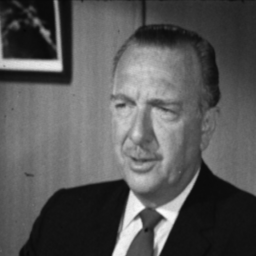
\includegraphics[width=0.4\textwidth]{gentelman_gray}
		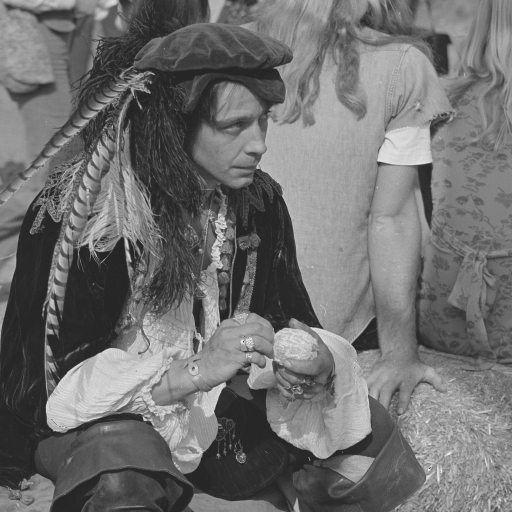
\includegraphics[width=0.4\textwidth]{pirate_gray}
	\end{center}
	\caption{Obrazy wejściowe (od lewej): obraz 1 (256x256), obraz 2 (512x512)}
\end{figure}

\begin{figure}[H]
	\begin{center}
		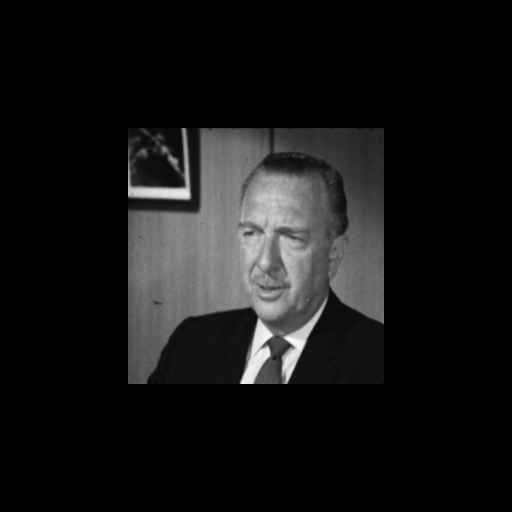
\includegraphics[width=0.4\textwidth]{gentelman_gray_unificationGeo_result}
		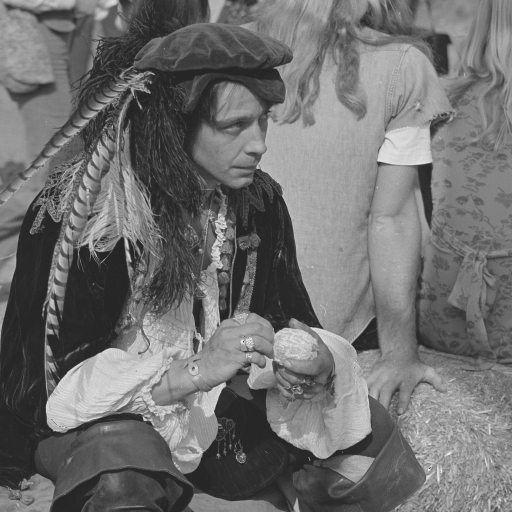
\includegraphics[width=0.4\textwidth]{pirate_gray_unificationGeo_result}
	\end{center}
	\caption{Obrazy wyjściowe (od lewej): obraz 1 (512x512), obraz 2 (512x512)}
\end{figure}

%\subsection*{Kod źródłowy}

\begin{lstlisting}[caption=Geometryczne ujednolicanie obrazów szarych]

def geometricGray(self, show = False):
	# najwieksza szerokosc sposrod dwuch obrazow
	width1 = self.im1.shape[1]
	width2 = self.im2.shape[1]
	maxWidth = width1 if width1 > width2 else width2

	# najwieksza wysokosc sposrod dwuch obrazow
	height1 = self.im1.shape[0]
	height2 = self.im2.shape[0]
	maxHeight = height1 if height1 > height2 else height2

	# alokacja pamieci na obrazy wynikowe
	resultImage1 = np.empty((maxHeight, maxWidth), dtype = np.uint8)
	resultImage2 = np.empty((maxHeight, maxWidth), dtype = np.uint8)

	# wspolrzedne poczatku rysowania obrazu 1 w srodku
	startWidthCoord = int(round((maxWidth - width1) / 2))
	startHeightCoord = int(round((maxHeight - height1) / 2))

	# wypelnienie obrazu czarny kolorem
	for i in range(0, maxHeight):
		for j in range(0, maxWidth):
			resultImage1[i, j] = 1

	# narysowanie wysrodkowanego obrazu
	for i in range(0, height1):
		for j in range(0, width1):
			resultImage1[i + startHeightCoord, j + startWidthCoord] = self.im1[i, j]

	# wspolrzedne poczatku rysowania obrazu 1 w srodku
	startWidthCoord = int(round((maxWidth - width2) / 2))
	startHeightCoord = int(round((maxHeight - height2) / 2))

	# wypelnienie obrazu czarnym kolorem
	for i in range(0, maxHeight):
		for j in range(0, maxWidth):
			resultImage2[i, j] = 1

	# narysowanie wysrodkowanego obrazu
	for i in range(0, height2):
		for j in range(0, width2):
			resultImage2[i + startHeightCoord, j + startWidthCoord] = self.im2[i, j]

	if show:
		self.show(Image.fromarray(resultImage1, "L"), Image.fromarray(resultImage2, "L"))
	self.save(resultImage1, self.im1Name, "unificationGeo")
	self.save(resultImage2, self.im2Name, "unificationGeo")

\end{lstlisting}


\newpage





\section{Ujednolicenie obrazów szarych rozdzielczościowe}
\subsection*{Opis algorytmu}
\hfill
\\\\
\indent 
Operacja ujednolicania obrazów dzieli się na dwa etapy. Pierwszym jest ujednolicenie geometryczne, drugim zaś ujednolicenie rozdzielczościowe.

Operacja rozdzielczościowego ujednolicenia obrazów następuje po ujednoliceniu geometrycznym i polega na wypełnieniu obrazu pikslami, a brakujące piksle powinny być zinterpolowane.
\begin{enumerate}
	\item Wypełnij cały obraz pikslami o znanej wartości zachowując pewien odstęp między nimi.
	\item Każdemu pikslowi o nieznanej wartości przypisz zinterpolowaną wartość znanych piksli z jego bezpośredniego otoczenia.
\end{enumerate}

\begin{figure}[H]
	\begin{center}
		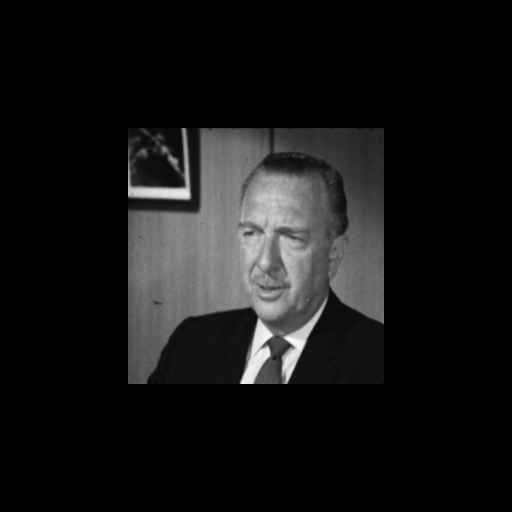
\includegraphics[width=0.35\textwidth]{gentelman_gray_unificationGeo_result}
		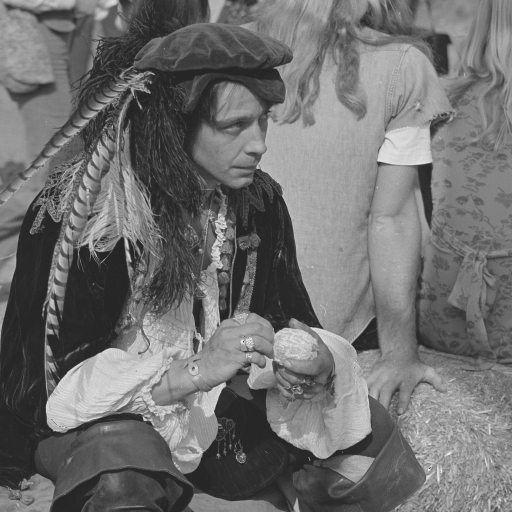
\includegraphics[width=0.35\textwidth]{pirate_gray_unificationGeo_result}
	\end{center}
	\caption{Obrazy wejściowe (od lewej): obraz 1 (512x512), obraz 2 (512x512)}
\end{figure}

\begin{figure}[H]
	\begin{center}
		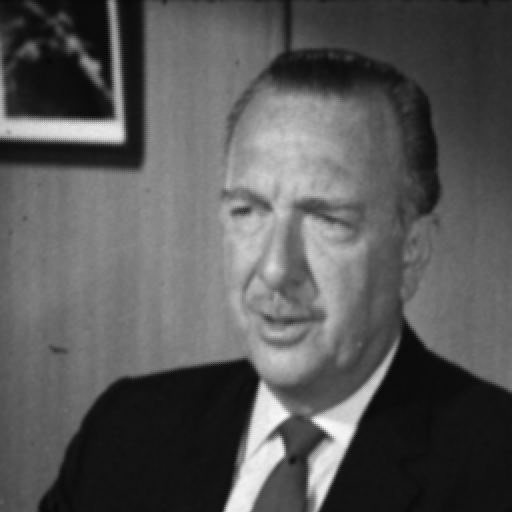
\includegraphics[width=0.35\textwidth]{gentelman_gray_unificationRas_result}
		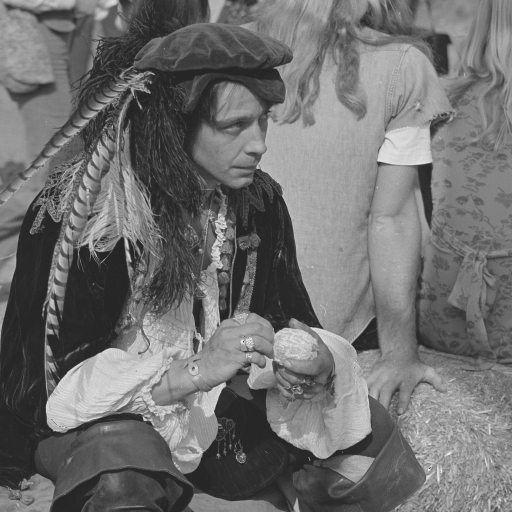
\includegraphics[width=0.35\textwidth]{pirate_gray_unificationRas_result}
	\end{center}
	\caption{Obrazy wyjściowe (od lewej): obraz 1 (512x512), obraz 2 (512x512)}
\end{figure}

%\subsection*{Kod źródłowy}

\begin{lstlisting}[caption=Rastrowe ujednolicanie obrazów szarych]

def rasterGray(self, show = False):
	# pierwszy jest ZAWSZE wiekszy
	width1 = self.im1.shape[1]
	width2 = self.im2.shape[1]
	
	height1 = self.im1.shape[0]
	height2 = self.im2.shape[0]
	
	scaleW = width1 / width2
	scaleH = height1 / height2
	
	# alokacja pamieci na obrazy wynikowe
	resultImage1 = np.zeros((height1, width1), dtype = np.uint8)
	resultImage2 = np.zeros((height1, width1), dtype = np.uint8)
	tmp = np.zeros((height1, width1), dtype = np.uint8)
	
	for i in range(height1):
		for j in range(width1):
			resultImage1[i, j] = self.im1[i, j]
	
	# wypelnianie
	count = 0
	for i in range(height2):
		for j in range(width2):
			if count == 0:
				resultImage2[int(scaleH*i), int(round(scaleW*j)) + 1] = self.im2[i, j]
				count += 1
			if count == 1:
				resultImage2[int(round(scaleH*i)) + 1, int(scaleW*j)] = self.im2[i, j]
				count = 0
	
	# interpolacja
	for i in range(height1):
		for j in range(width1):
			value = 0
			n = 0
			tmp[i, j] = resultImage2[i, j]
			if resultImage2[i, j] < 1:
				for iOff in range(-1, 2):
					for jOff in range(-1, 2):
						iSafe = i if ((i + iOff) > (height1 - 2)) | ((i + iOff) < 0) else (i + iOff)
						jSafe = j if ((j + jOff) > (width1 - 2)) | ((j + jOff) < 0) else (j + jOff)
						if resultImage2[iSafe, jSafe] > 0:
							value += resultImage2[iSafe, jSafe]
							n += 1
				tmp[i, j] = value / n
				resultImage2[i, j] = tmp[i, j]
	
	if show:
		self.show(Image.fromarray(resultImage1, "L"), Image.fromarray(resultImage2, "L"))
	self.save(resultImage1, self.im1Name, "unificationRas")
	self.save(resultImage2, self.im2Name, "unificationRas")

\end{lstlisting}

\newpage







\section{Ujednolicenie obrazów RGB geometryczne}
\subsection*{Opis algorytmu}
\hfill
\\\\
\indent 
Operacja ujednolicania obrazów dzieli się na dwa etapy. Pierwszym jest ujednolicenie geometryczne, drugim zaś ujednolicenie rozdzielczościowe.

Operacja geometrycznego ujednolicenia obrazów polega na doprowadzeniu obydwu obrazów do takiej samej liczby wierszy piksli w każdym obrazie i takiej samej liczby kolumn piksli w każdym obrazie.
\begin{enumerate}
	\item Wybierz największą wysokość i największą szerokość z dwuch obrazów.
	\item Jeśli dany obraz ma mniejszą szerokość albo wysokość, wypełnij różnicę pikslami o wartości 1 dla każdego z kanałów R, G i B (aby uniknąć dzielenia przez 0).
\end{enumerate}

\begin{figure}[H]
	\begin{center}
		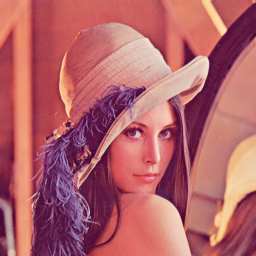
\includegraphics[width=0.4\textwidth]{lena_color}
		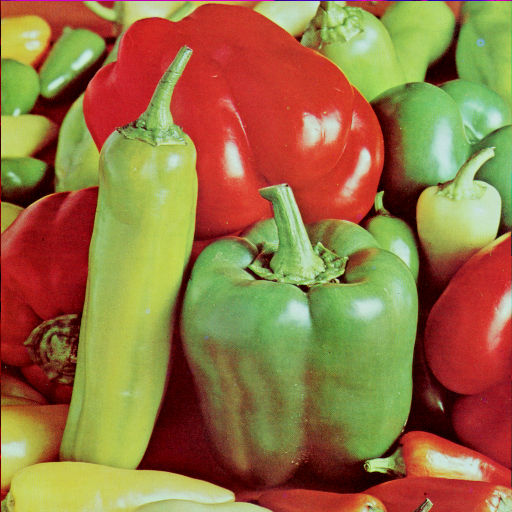
\includegraphics[width=0.4\textwidth]{peppers_color}
	\end{center}
	\caption{Obrazy wejściowe (od lewej): obraz 1 (256x256), obraz 2 (512x512)}
\end{figure}

\begin{figure}[H]
	\begin{center}
		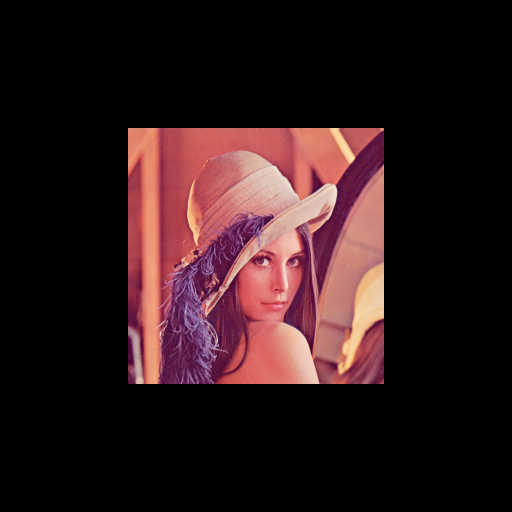
\includegraphics[width=0.4\textwidth]{lena_color_unificationGeo_result}
		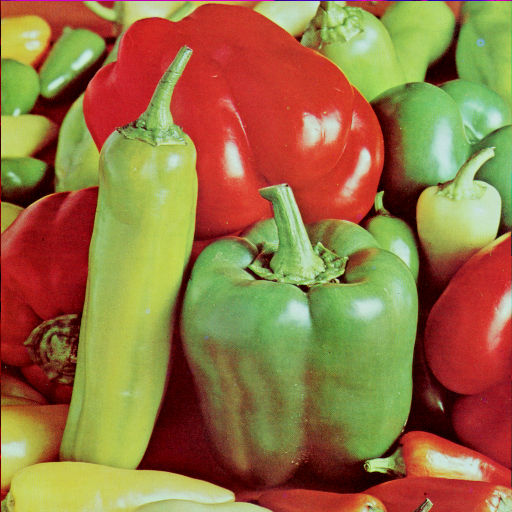
\includegraphics[width=0.4\textwidth]{peppers_color_unificationGeo_result}
	\end{center}
	\caption{Obrazy wyjściowe (od lewej): obraz 1 (512x512), obraz 2 (512x512)}
\end{figure}

%\subsection*{Kod źródłowy}

\begin{lstlisting}[caption=Geometryczne ujednolicanie obrazów barwnych]

def geometricColor(self, show = False):
	# najwieksza szerokosc sposrod dwuch obrazow
	width1 = self.im1.shape[1]
	width2 = self.im2.shape[1]
	maxWidth = width1 if width1 > width2 else width2
	
	# najwieksza wysokosc sposrod dwuch obrazow
	height1 = self.im1.shape[0]
	height2 = self.im2.shape[0]
	maxHeight = height1 if height1 > height2 else height2
	
	# alokacja pamieci na obrazy wynikowe
	resultImage1 = np.empty((maxHeight, maxWidth, 3), dtype = np.uint8)
	resultImage2 = np.empty((maxHeight, maxWidth, 3), dtype = np.uint8)
	
	# wspolrzedne poczatku rysowania obrazu 1 w srodku
	startWidthCoord = int(round((maxWidth - width1) / 2))
	startHeightCoord = int(round((maxHeight - height1) / 2))
	
	# wypelnienie obrazu czarnym kolorem
	for i in range(0, maxHeight):
		for j in range(0, maxWidth):
			resultImage1[i, j] = (1, 1, 1)
	
	# narysowanie wysrodkowanego obrazu
	for i in range(0, height1):
		for j in range(0, width1):
			resultImage1[i + startHeightCoord, j + startWidthCoord] = self.im1[i, j]
	
	# wspolrzedne poczatku rysowania obrazu 1 w srodku
	startWidthCoord = int(round((maxWidth - width2) / 2))
	startHeightCoord = int(round((maxHeight - height2) / 2))
	
	# wypelnienie obrazu czarnym kolorem
	for i in range(0, maxHeight):
		for j in range(0, maxWidth):
			resultImage2[i, j] = (1, 1, 1)

	# narysowanie wysrodkowanego obrazu
	for i in range(0, height2):
		for j in range(0, width2):
			resultImage2[i + startHeightCoord, j + startWidthCoord] = self.im2[i, j]
	
	if show:
		self.show(Image.fromarray(resultImage1, "RGB"), Image.fromarray(resultImage2, "RGB"))
	self.save(resultImage1, self.im1Name, "unificationGeo")
	self.save(resultImage2, self.im2Name, "unificationGeo")
\end{lstlisting}

\newpage





\section{Ujednolicenie obrazów RGB rozdzielczościowe}
\subsection*{Opis algorytmu}
\hfill
\\\\
\indent 
Operacja ujednolicania obrazów dzieli się na dwa etapy. Pierwszym jest ujednolicenie geometryczne, drugim zaś ujednolicenie rozdzielczościowe.

Operacja rozdzielczościowego ujednolicenia obrazów następuje po ujednoliceniu geometrycznym i polega na wypełnieniu obrazu pikslami, a brakujące piksle powinny być zinterpolowane.
\begin{enumerate}
	\item Wypełnij cały obraz pikslami o znanej wartości zachowując pewien odstęp między nimi.
	\item Każdemu pikslowi o nieznanej wartości przypisz zinterpolowaną wartość (dla każdego z kanałów R, G, B) znanych piksli z jego bezpośredniego otoczenia.
\end{enumerate}

\begin{figure}[H]
	\begin{center}
		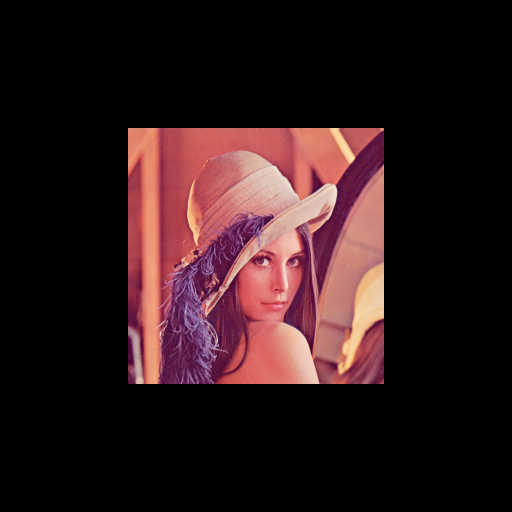
\includegraphics[width=0.4\textwidth]{lena_color_unificationGeo_result}
		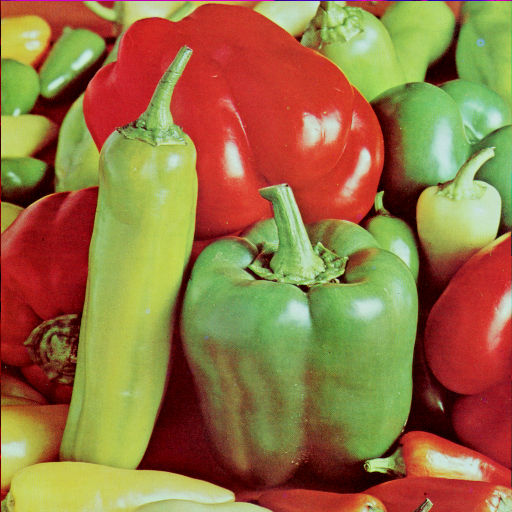
\includegraphics[width=0.4\textwidth]{peppers_color_unificationGeo_result}
	\end{center}
	\caption{Obrazy wejściowe (od lewej): obraz 1 (512x512), obraz 2 (512x512)}
\end{figure}

\begin{figure}[H]
	\begin{center}
		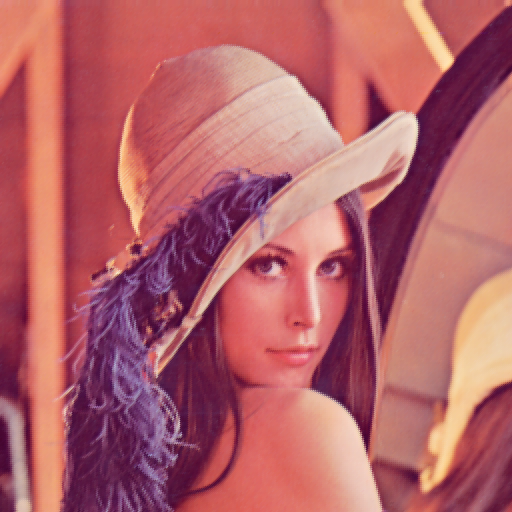
\includegraphics[width=0.4\textwidth]{lena_color_unificationRas_result}
		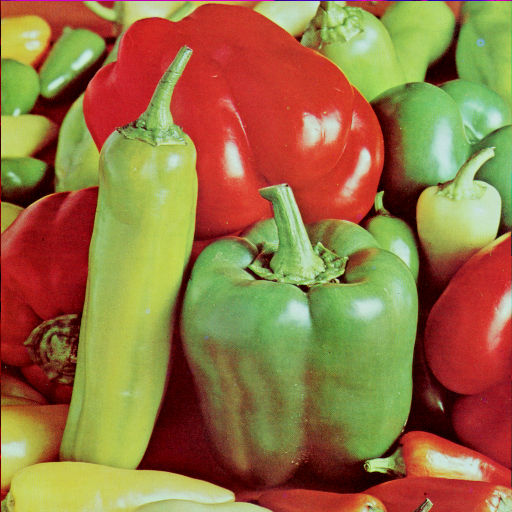
\includegraphics[width=0.4\textwidth]{peppers_color_unificationRas_result}
	\end{center}
	\caption{Obrazy wyjściowe (od lewej): obraz 1 (512x512), obraz 2 (512x512)}
\end{figure}

%\subsection*{Kod źródłowy}

\begin{lstlisting}[caption=Rastrowe ujednolicanie obrazów barwnych]

def rasterColor(self, show = False):
	# pierwszy jest ZAWSZE wiekszy
	width1 = self.im1.shape[1]
	width2 = self.im2.shape[1]
	
	height1 = self.im1.shape[0]
	height2 = self.im2.shape[0]
	
	scaleW = width1 / width2
	scaleH = height1 / height2
	
	# alokacja pamieci na obrazy wynikowe
	resultImage1 = np.zeros((height1, width1, 3), dtype = np.uint8)
	resultImage2 = np.zeros((height1, width1, 3), dtype = np.uint8)
	tmp = np.zeros((height1, width1, 3), dtype = np.uint8)
	
	for i in range(height1):
		for j in range(width1):
			resultImage1[i, j] = self.im1[i, j]
	
	# wypelnianie
	count = 0
	for i in range(height2):
		for j in range(width2):
			if count == 0:
				resultImage2[int(scaleH*i), int(round(scaleW*j)) + 1] = self.im2[i, j]
				count += 1
			if count == 1:
				resultImage2[int(round(scaleH*i)) + 1, int(scaleW*j)] = self.im2[i, j]
				count = 0
	
	# interpolacja
	for i in range(height1):
		for j in range(width1):
			r, g, b = 0, 0, 0
			n = 0
			tmp[i, j] = resultImage2[i, j]
			if (resultImage2[i, j][0] < 1) & (resultImage2[i, j][1] < 1) & (resultImage2[i, j][2] < 1):
				for iOff in range(-1, 2):
					for jOff in range(-1, 2):
						iSafe = i if ((i + iOff) > (height1 - 2)) | ((i + iOff) < 0) else (i + iOff)
						jSafe = j if ((j + jOff) > (width1 - 2)) | ((j + jOff) < 0) else (j + jOff)
						if (resultImage2[iSafe, jSafe][0] > 0) | (resultImage2[iSafe, jSafe][1] > 0) | (resultImage2[iSafe, jSafe][2] > 0):
							r += resultImage2[iSafe, jSafe][0]
							g += resultImage2[iSafe, jSafe][1]
							b += resultImage2[iSafe, jSafe][2]
							n += 1
			tmp[i, j] = (r/n, g/n, b/n)
			resultImage2[i, j] = tmp[i, j]
	
	if show:
		self.show(Image.fromarray(resultImage1, "RGB"), Image.fromarray(resultImage2, "RGB"))
	self.save(resultImage1, self.im1Name, "unificationRas")
	self.save(resultImage2, self.im2Name, "unificationRas")

\end{lstlisting}










\chapter{Operacje sumowania arytmetycznego obrazów szarych}
1. Sumowanie (określonej) stałej z obrazem oraz dwóch obrazów
2. Mnożenie obrazu przez zadaną liczbę oraz przez inny obraz
3. Mieszanie obrazów z określonym współczynnikiem
4. Potęgowanie obrazu (z zadaną potęgą)
5. Dzielenie obrazu przez (zadaną) liczbę oraz przez inny obraz
6. Pierwiastkowanie obrazu
7. Logarytmowanie obrazu

\chapter{Operacje sumowania arytmetycznego obrazów barwowych}
1. sumowanie (określonej) stałej z obrazem oraz dwóch obrazów
2. mnożenie obrazu przez zadaną liczbę oraz przez inny obraz
3. mieszanie obrazów z określonym współczynnikiem
4. potęgowanie obrazu (z zadaną potęgą)
5. dzielenie obrazu przez (zadaną) liczbę oraz przez inny obraz
6. pierwiastkowanie obrazu
7. logarytmowanie obrazu

\chapter{Operacje geometryczne na obrazie}
1. przemieszczenie obrazu o zadany wektor
2. jednorodne i niejednorodne skalowanie obrazu
3. obracanie obrazu o dowolny kąt
4. symetrie względem osi układu i zadanej prostej
5. wycinanie fragmentów obrazu
6. kopiowanie fragmentów obrazów

\chapter{Operacje na histogramie obrazu szarego}
\pagebreak
\section{Obliczanie histogramu}
\subsection*{Opis algorytmu}
\hfill
\\\\
\indent 
Histogram obrazu szarego jest wykresem częstości występowania wartości szarości piksli w obrazie tj.
przyporządkowuje liczbę piskli do danego poziomu szarości.\newline
\begin{enumerate}
	\item Zaalokuj tablicę 256 elementową (tyle, ile poziomów szarości w obrazie)
	\item Dla każdego piskla:
	\item Zinkrementuj element tablicy o indeksie równym pozionie szarości danego piskla
\end{enumerate}

\begin{figure}[H]
	\begin{center}
		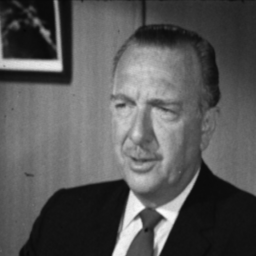
\includegraphics[width=0.4\textwidth]{gentelman_gray}
		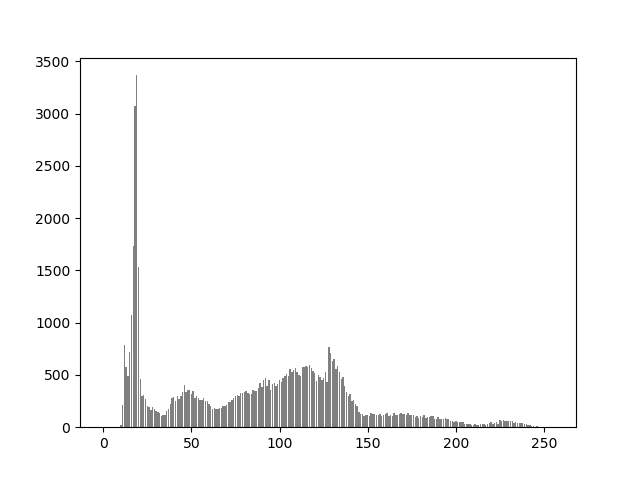
\includegraphics[width=0.4\textwidth]{gentelman_gray_histogram}
	\end{center}
	\caption{Obraz szary, histogram szarości tego obrazu}
\end{figure}

\begin{figure}[H]
	\begin{center}
		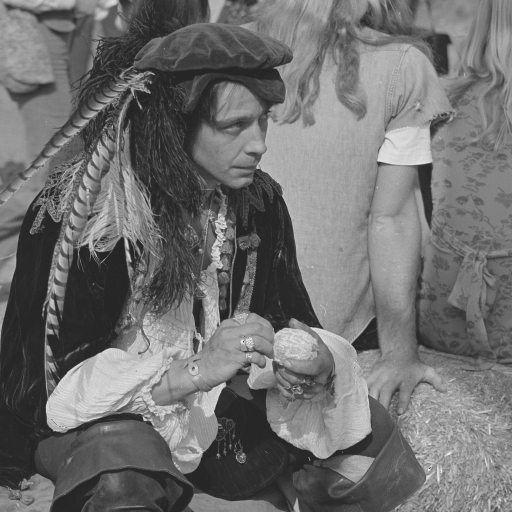
\includegraphics[width=0.4\textwidth]{pirate_gray}
		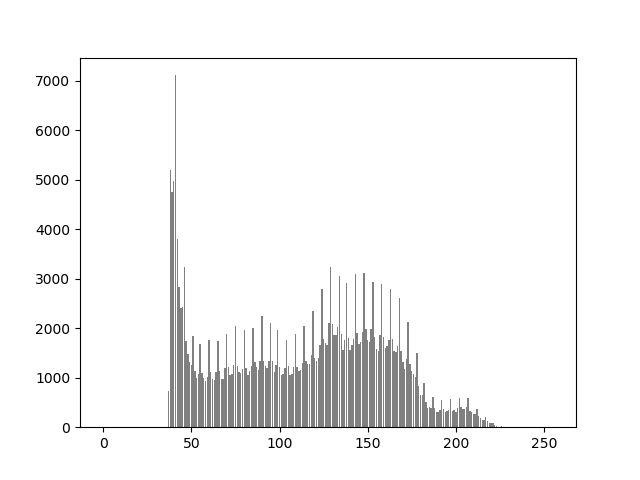
\includegraphics[width=0.4\textwidth]{pirate_gray_histogram}
	\end{center}
	\caption{Obraz szary, histogram szarości tego obrazu}
\end{figure}
\newpage

%\subsection*{Kod źródłowy}

\begin{lstlisting}[caption=Obliczanie histogramu]
	
def calculate(self, plot = False, image = None):
	if image is None:
		image = self.im
	
	width = image.shape[1]      # szereoksc
	height = image.shape[0]     # wysokosc
	hist = [0] * 256            # hostogram szarosci
	
	for i in range(height):
		for j in range(width):
			bin = image[i, j]   # odcien szarosci
			hist[bin] += 1
	
	if plot:
		# tablica [0, 1, ... , 254, 255]
		bins = np.arange(256)
		self.plotHistogram(bins, hist)
	
	return hist
	
\end{lstlisting}

\newpage





\section{Przemieszczanie histogramu}
\subsection*{Opis algorytmu}
\hfill
\\\\
\indent Przemieszczenie histogramu polega na dodaniu lub odjęciu tej samej wartości od poziomu szarości każdego piksla w obrazie.
W rezultacie obraz jest odpowiednio równomiernie rozjaśniony bądź przyciemniony.
Nie można przekroczyć przyjętego zakresu poziomów szarości.
\begin{enumerate}
	\item Do każdej wartości piksla dodaj podaną stałą o którą chcesz przemieścić histogram.
	\item Jeśli wartość piksla po operacji dodawania wykracza poza zakres 255:
	\item Przypisz jej wartość 255.
	\item Jeśli wartość piksla po operacji dodawania jest mniejsza od 0:
	\item Przypisz jej wartość 0.
\end{enumerate}

\begin{figure}[H]
	\begin{center}
		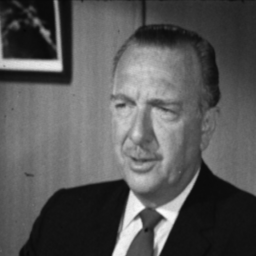
\includegraphics[width=0.4\textwidth]{gentelman_gray}
		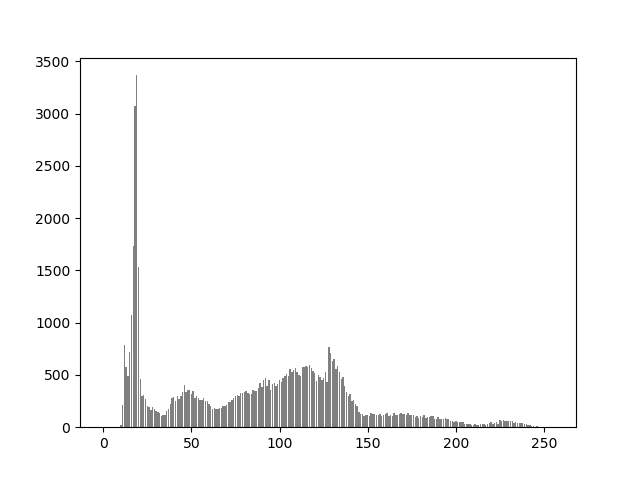
\includegraphics[width=0.4\textwidth]{gentelman_gray_histogram}
	\end{center}
	\caption{Obraz szary wejściowy, histogram szarości tego obrazu}
\end{figure}

\begin{figure}[H]
	\begin{center}
		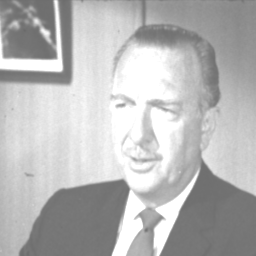
\includegraphics[width=0.4\textwidth]{gentelman_gray_moveHist_result}
		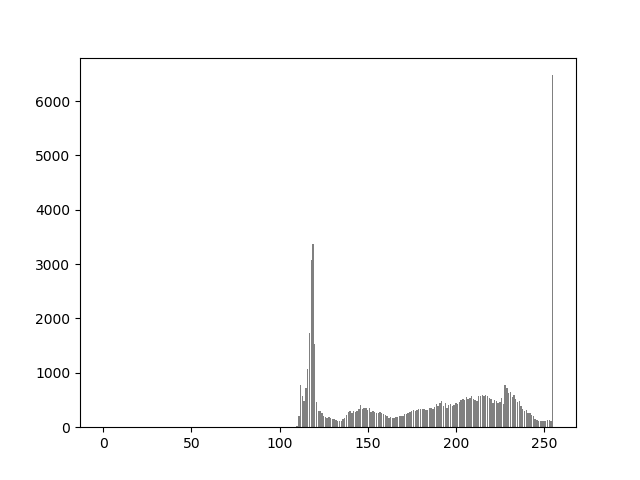
\includegraphics[width=0.4\textwidth]{gentelman_gray_moveHist_histogram}
	\end{center}
	\caption{Obraz szary przesunięty o 100, histogram szarości tego obrazu}
\end{figure}

\begin{figure}[t]
	\begin{center}
		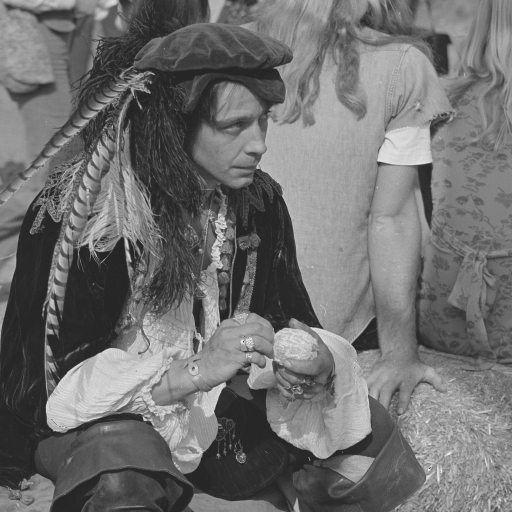
\includegraphics[width=0.4\textwidth]{pirate_gray}
		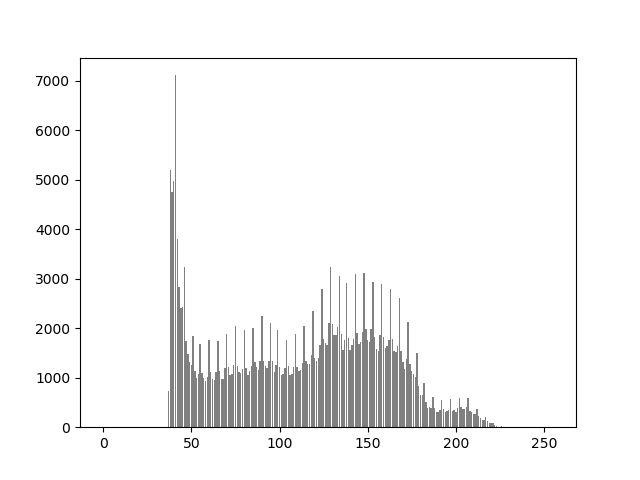
\includegraphics[width=0.4\textwidth]{pirate_gray_histogram}
	\end{center}
	\caption{Obraz szary wejściowy, histogram szarości tego obrazu}
\end{figure}

\begin{figure}[H]
	\begin{center}
		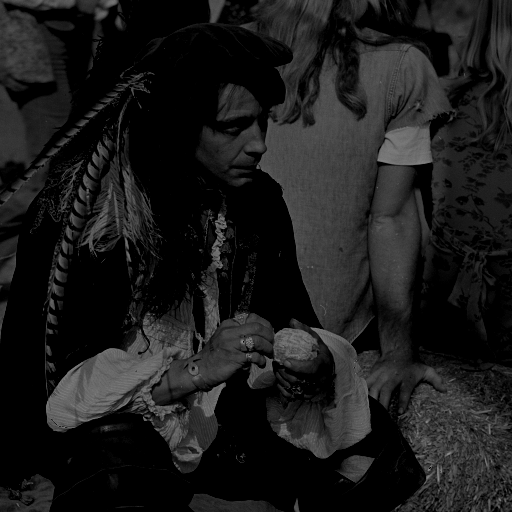
\includegraphics[width=0.4\textwidth]{pirate_gray_moveHist_result}
		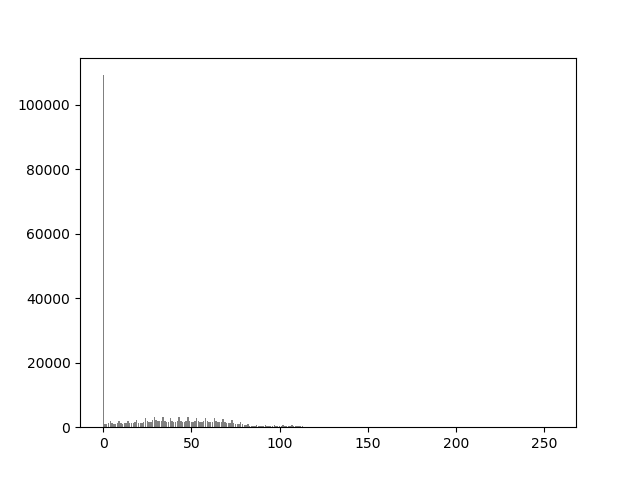
\includegraphics[width=0.4\textwidth]{pirate_gray_moveHist_histogram}
	\end{center}
	\caption{Obraz szary pryesunięty o -100, histogram szarości tego obrazu}
\end{figure}



%\subsection*{Kod źródłowy}

\begin{lstlisting}[caption=Przemieszczanie histogramu]
def move(self, const = 0, show = False, plot = False):
	width = self.im.shape[1]    # szereoksc
	height = self.im.shape[0]   # wysokosc
	
	# alokacja pamieci na obraz wynikowy
	resultImage = np.empty((height, width), dtype=np.uint8)
	
	# przemieszczanie
	for i in range(height):
		for j in range(width):
			value = int(self.im[i, j]) + const
			if value < 0:
				value = 0
			elif value > 255:
				value = 255
			resultImage[i, j] = value
	
	if show:
		self.show(Image.fromarray(resultImage, "L"))
	self.calculate(plot, resultImage)
	self.save(resultImage, self.imName, "moveHist")
\end{lstlisting}

\newpage





\section{Rozciąganie histogramu}
\subsection*{Opis algorytmu}
\hfill
\\\\
\indent Rozciągania histogramu dokonuje się na obrazie, którego poziomy szarości nie są rozpięte na cały możliwy zakres np.
[51, 233]. Operacja rozciągnięcia histogramu rozciągnie histogram tak, aby był rozpięty na cały możliwy zakres poziomów szarości np. [0, 255].
\begin{enumerate}
	\item Znajdź w obrazie największą($max$) i najmniejszą($min$) wartość piksla
	\item Dla każdego piksla:
	\item Oblicz nową wartość piskla stosując wzór:\\
	\centerline{$P_n = 255$ $//$ $(max - min) * (P_o - min)$.}
	W taki sposób, jeśli odcienie szarości obrazu wejściowego były w zakresie
	np. $[12, 239]$, po operacji rozciągania histogramu, odcienie szarości będą w zakresie\\
	$[0, 255]$
\end{enumerate}

\begin{figure}[H]
	\begin{center}
		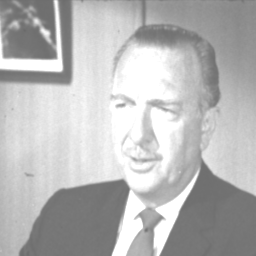
\includegraphics[width=0.35\textwidth]{gentelman_gray_moveHist_result}
		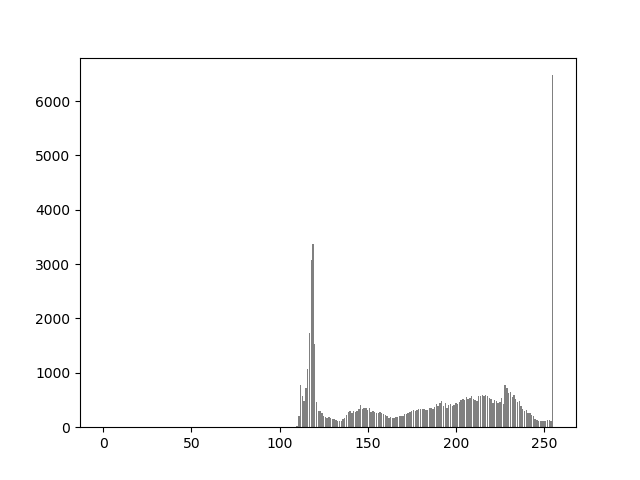
\includegraphics[width=0.35\textwidth]{gentelman_gray_moveHist_histogram}
	\end{center}
	\caption{Obraz wejściowy, histogram szarości tego obrazu}
\end{figure}

\begin{figure}[H]
	\begin{center}
		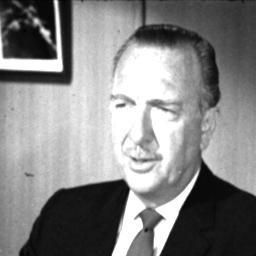
\includegraphics[width=0.35\textwidth]{gentelman_gray_stretchHist_result}
		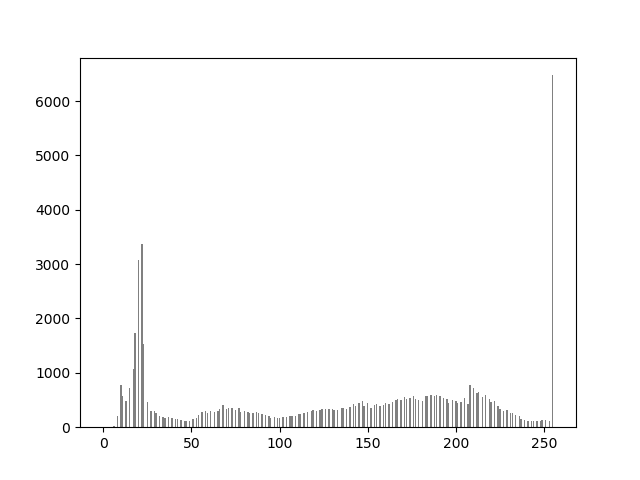
\includegraphics[width=0.35\textwidth]{gentelman_gray_stretchHist_histogram}
	\end{center}
	\caption{Obraz po rozciągnięciu, histogram szarości tego obrazu}
\end{figure}

\begin{figure}[H]
	\begin{center}
		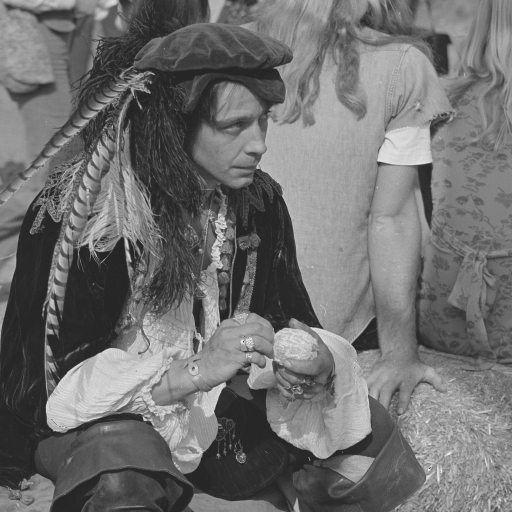
\includegraphics[width=0.35\textwidth]{pirate_gray}
		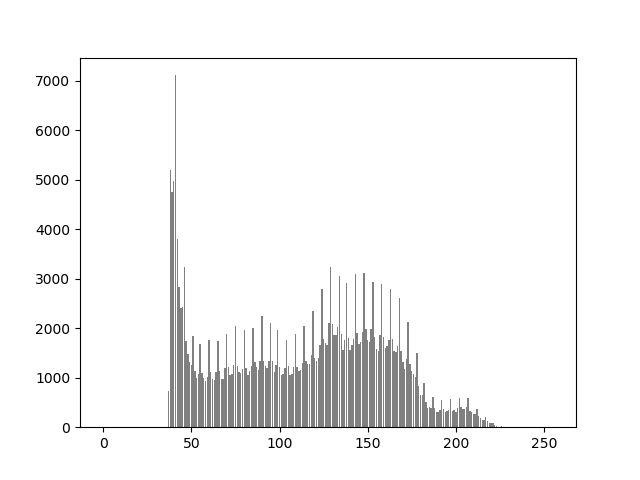
\includegraphics[width=0.35\textwidth]{pirate_gray_histogram}
	\end{center}
	\caption{Obraz wejściowy, histogram szarości tego obrazu}
\end{figure}

\begin{figure}[H]
	\begin{center}
		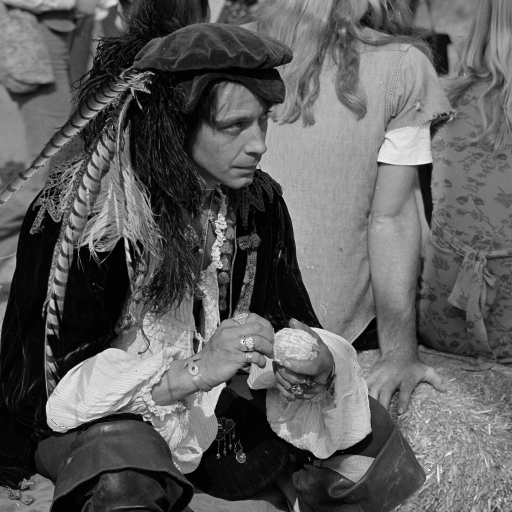
\includegraphics[width=0.35\textwidth]{pirate_gray_stretchHist_result}
		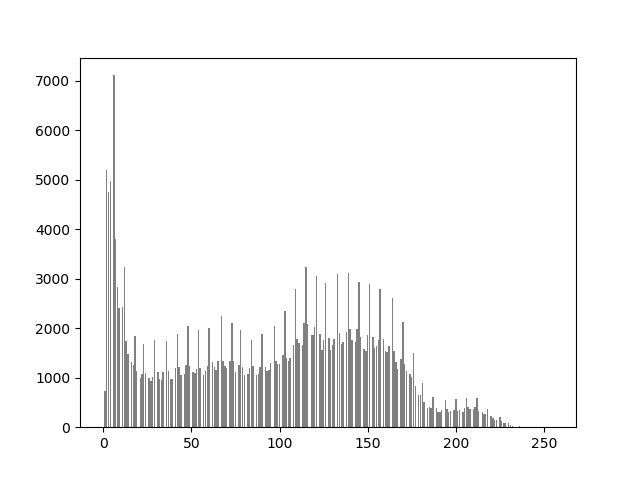
\includegraphics[width=0.35\textwidth]{pirate_gray_stretchHist_histogram}
	\end{center}
	\caption{Obraz po rozciągnięciu, histogram szarości tego obrazu}
\end{figure}

%\subsection*{Kod źródłowy}

\begin{lstlisting}[caption=Rozciąganie histogramu]
def stretch(self, show = False, plot = False):
	width = self.im.shape[1]    # szereoksc
	height = self.im.shape[0]   # wysokosc
	
	# alokacja pamieci na obraz wynikowy
	resultImage = np.empty((height, width), dtype=np.uint8)
	for i in range(height):
		for j in range(width):
			resultImage[i, j] = self.im[i, j]
	
	# wartosc min i max w obrazie
	maxValue = 0
	minValue = 255
	while maxValue != 255:
		# wartosci max i min w obrazie
		for i in range(height):
			for j in range(width):
				currValue = resultImage[i, j]
				maxValue = max(maxValue, currValue)
				minValue = min(minValue, currValue)
	
	# rozciaganie
	for i in range(height):
		for j in range(width):
			pix = resultImage[i, j]
			resultImage[i, j] = ((255 / (maxValue - minValue)) * (pix - minValue))
	
	if show:
		self.show(Image.fromarray(resultImage, "L"))
	self.calculate(plot, resultImage)
	self.save(resultImage, self.imName, "stretchHist")
\end{lstlisting}

\newpage





\section{Progowanie lokalne}
\subsection*{Opis algorytmu}
\hfill
\\\\
\indent Progowanie lokalne oblicza wartość progową dla każdego piksla z osobna. Jest to jedna z metod binaryzacji obrazu, która w wyniku dokładniej odwzorowuje kształt obiektu na obrazie.
\begin{enumerate}
	\item Zdefiniuj wielkość otoczenia piksla (musi być nieparzysta, po to, aby mógł istnieć piksel środkowy).
	\item Dla każdego piskla:
	\item Oblicz wartość progową jako średnią wartość piksli w otoczeniu danego piksla.
	\item Jeśli wartość piksla środkowego jest $< 0$:
	\item Przypisz mu wartość $0$.
	\item W przeciwnym przypadku przypisz mu wartość $255$.
\end{enumerate}

\begin{figure}[H]
	\begin{center}
		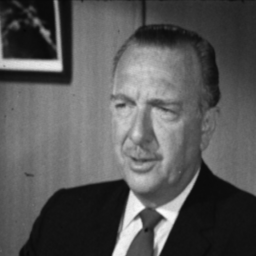
\includegraphics[width=0.37\textwidth]{gentelman_gray}
		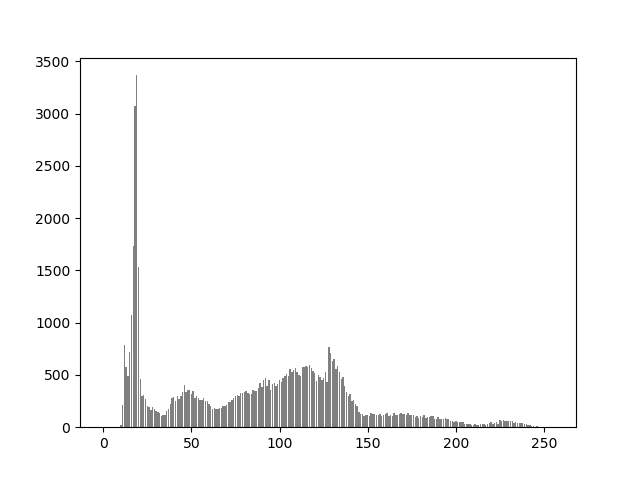
\includegraphics[width=0.37\textwidth]{gentelman_gray_histogram}
	\end{center}
	\caption{Obraz wejściowy, histogram szarości tego obrazu}
\end{figure}

\begin{figure}[H]
	\begin{center}
		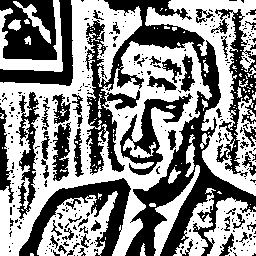
\includegraphics[width=0.37\textwidth]{gentelman_gray_locThreshold_result}
		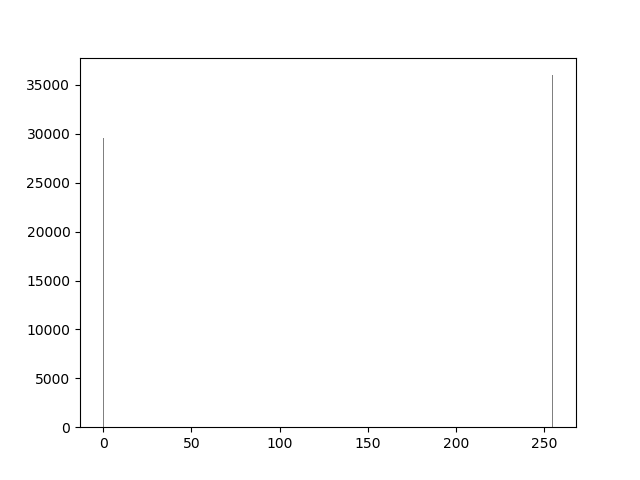
\includegraphics[width=0.37\textwidth]{gentelman_gray_locThreshold_histogram}
	\end{center}
	\caption{Obraz po progowaniu z parametrem 20, histogram szarości tego obrazu}
\end{figure}

\begin{figure}[H]
	\begin{center}
		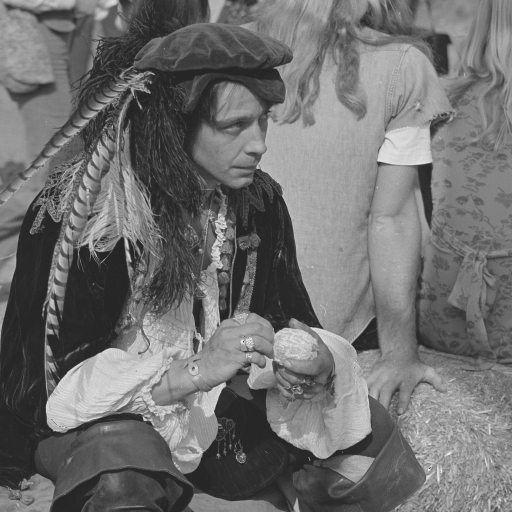
\includegraphics[width=0.4\textwidth]{pirate_gray}
		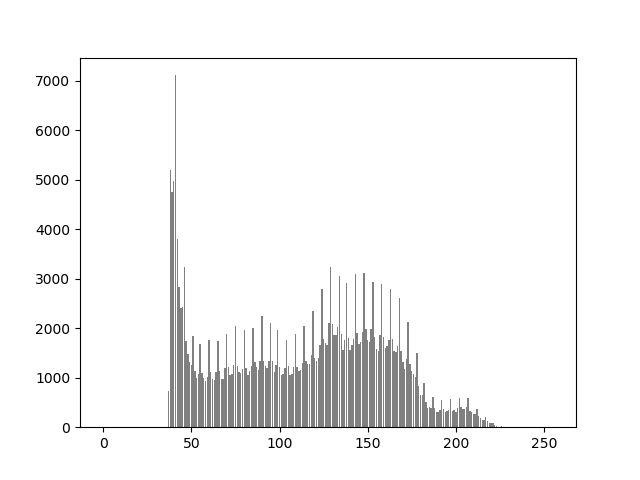
\includegraphics[width=0.4\textwidth]{pirate_gray_histogram}
	\end{center}
	\caption{Obraz wejściowy, histogram szarości tego obrazu}
\end{figure}

\begin{figure}[H]
	\begin{center}
		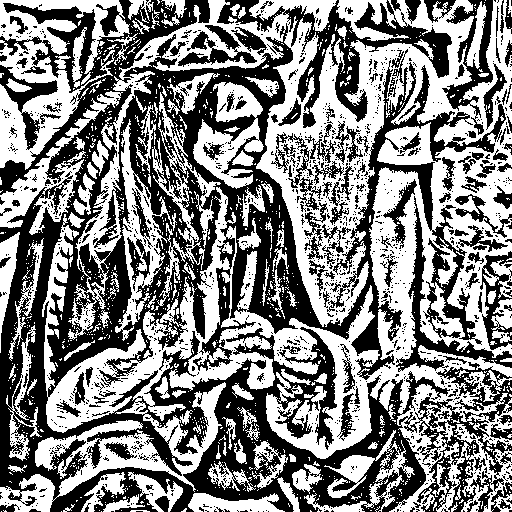
\includegraphics[width=0.4\textwidth]{pirate_gray_locThreshold_result}
		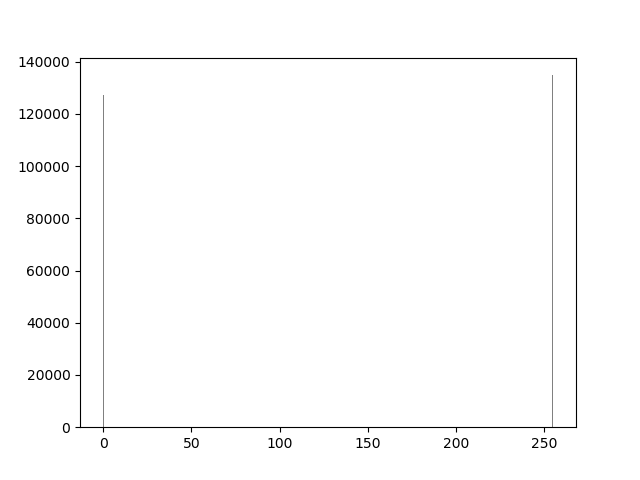
\includegraphics[width=0.4\textwidth]{pirate_gray_locThreshold_histogram}
	\end{center}
	\caption{Obraz po progowaniu z parametrem 20, histogram szarości tego obrazu}
\end{figure}

%\subsection*{Kod źródłowy}

\begin{lstlisting}[caption=Progowanie lokalne]
def localThreshold(self, dim = 3, show = False, plot = False):
	width = self.im.shape[1]    # szereoksc
	height = self.im.shape[0]   # wysokosc
	l, r = -(int(round(dim / 2))), int(round(dim / 2) + 1)  # wsp. sasiadow
	
	# alokacja pamieci na obraz wynikowy
	resultImage = np.empty((height, width), dtype=np.uint8)
	
	# progowanie lokalne
	for i in range(height):
		for j in range(width):
		n = 0
		threshold = 0
		currPix = self.im[i, j]
		for iOff in range(l, r):
			for jOff in range(l, r):
				iSafe = i if ((i + iOff) > (height + l)) else (i + iOff)
				jSafe = j if ((j + jOff) > (width + l)) else (j + jOff)
				threshold += self.im[iSafe, jSafe]
				n += 1
		threshold = int(round(threshold / n))
		resultImage[i, j] = 0 if (currPix < threshold) else 255
	
	if show:
		self.show(Image.fromarray(resultImage, "L"))
	self.calculate(plot, resultImage)
	self.save(resultImage, self.imName, "locThreshold")
\end{lstlisting}

\newpage
\clearpage




\section{Progowanie globalne}
\subsection*{Opis algorytmu}
\hfill
\\\\
\indent Progowanie globalne jest jedną z metod binaryzacji obrazu. Wartość progowa jest ustalana globalnie biorąc pod uwagę wartość każdego piklsla w obrazie, po czym stosując wyliczony próg aby nadać nową wartość każdemu poikslowi obraz w wyniku jest binarny.
\begin{enumerate}
	\item Oblicz wartość progową $T$, jako średnią wartość z wszystkich piskli w obrazie
	\item Dla każdego piskla:
	\item Jeśli wartość danego piskla jest $< T$:
	\item przypisz mu wartość $0$.
	\item W przeciwnym przypadku przypisz mu wartość 255.
\end{enumerate}

\begin{figure}[H]
	\begin{center}
		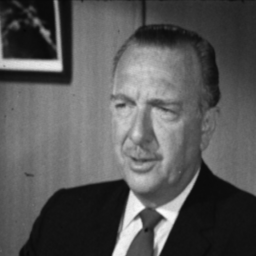
\includegraphics[width=0.4\textwidth]{gentelman_gray}
		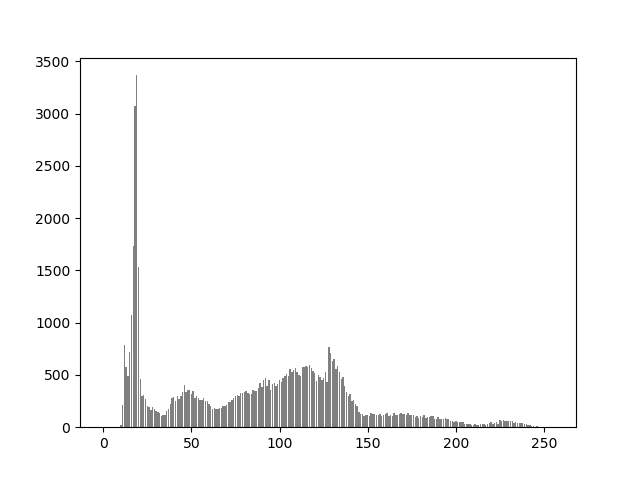
\includegraphics[width=0.4\textwidth]{gentelman_gray_histogram}
	\end{center}
	\caption{Obraz wejściowy, histogram szarości tego obrazu}
\end{figure}

\begin{figure}[H]
	\begin{center}
		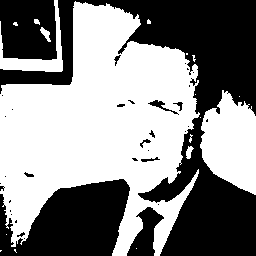
\includegraphics[width=0.4\textwidth]{gentelman_gray_globThreshold_result}
		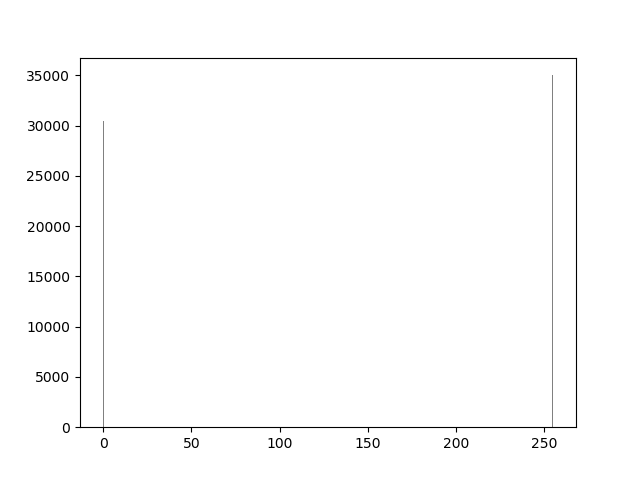
\includegraphics[width=0.4\textwidth]{gentelman_gray_globThreshold_histogram}
	\end{center}
	\caption{Obraz po progowaniu z parametrem 20, histogram szarości tego obrazu}
\end{figure}

\begin{figure}[H]
	\begin{center}
		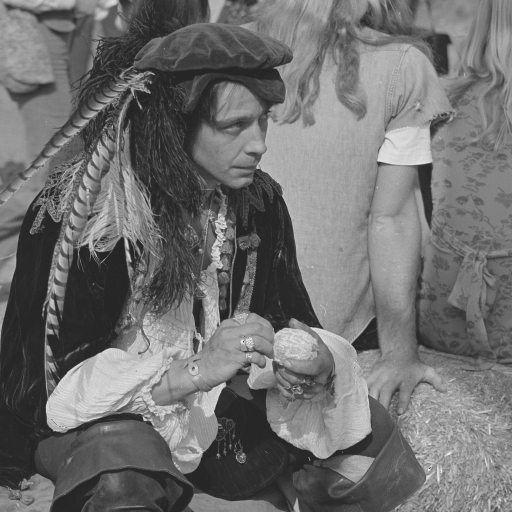
\includegraphics[width=0.4\textwidth]{pirate_gray}
		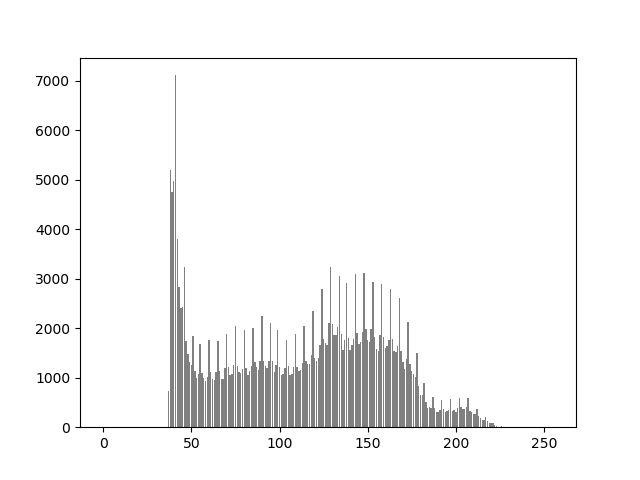
\includegraphics[width=0.4\textwidth]{pirate_gray_histogram}
	\end{center}
	\caption{Obraz wejściowy, histogram szarości tego obrazu}
\end{figure}

\begin{figure}[H]
	\begin{center}
		\includegraphics[width=0.4\textwidth]{pirate_gray_globThreshold_result}
		\includegraphics[width=0.4\textwidth]{pirate_gray_globThreshold_histogram}
	\end{center}
	\caption{Obraz po progowaniu z parametrem 20, histogram szarości tego obrazu}
\end{figure}

%\subsection*{Kod źródłowy}
\begin{lstlisting}[caption=Progowanie globalne]
def globalThreshold(self, show = False, plot = False):
	width = self.im.shape[1]    # szereoksc
	height = self.im.shape[0]   # wysokosc
	
	# alokacja pamieci na obraz wynikowy
	resultImage = np.empty((height, width), dtype=np.uint8)
	
	# prog globalny
	threshold = 0
	n = 0
	for i in range(height):
		for j in range(width):
		threshold += self.im[i, j]
		n += 1
		threshold = int(round(threshold / n))
	
	# binaryzacja
	for i in range(height):
		for j in range(width):
			resultImage[i, j] = 0 if (self.im[i, j] < threshold) else 255
	
	if show:
		self.show(Image.fromarray(resultImage, "L"))
	self.calculate(plot, resultImage)
	self.save(resultImage, self.imName, "globThreshold")
\end{lstlisting}
\newpage






\chapter{Operacje na histogramie obrazu barwowego}
\pagebreak
\section{Obliczanie histogramu}
\subsection*{Opis algorytmu}
\hfill
\\\\
\indent Histogram obrazu barwnego jest wykresem częstości występowania wartości barwy piksli w obrazie tj.
przyporządkowuje liczbę piskli do danego poziomu barwy.\newline
\begin{enumerate}
	\item Zaalokuj 3 tablice 256 elementowe (tyle, ile poziomów barw w obrazie)
	\item Dla każdego piskla:
	\item Dla każdej barwy:
	\item Zinkrementuj element tablicy danej barwy o indeksie równym poziomie tej barwy danego piskla
\end{enumerate}

\begin{figure}[H]
	\begin{center}
		\includegraphics[width=0.4\textwidth]{lena_color}
		\includegraphics[width=0.4\textwidth]{lena_color_histogram}
	\end{center}
	\caption{Obraz barwny, histogram barw tego obrazu}
\end{figure}

\begin{figure}[H]
	\begin{center}
		\includegraphics[width=0.4\textwidth]{peppers_color}
		\includegraphics[width=0.4\textwidth]{peppers_color_histogram}
	\end{center}
	\caption{Obraz barwny, histogram barw tego obrazu}
\end{figure}
\pagebreak

%\subsection*{Kod źródłowy}

\begin{lstlisting}[caption=Obliczanie histogramu]
def calculate(self, plot = False, image = None):
	if image is None:
	image = self.im
	
	width = image.shape[1]      # szerokosc
	height = image.shape[0]     # wysokosc
	hist = [0] * 3              # histogram RGB
	hist[0] = [0] * 256         # histogram R
	hist[1] = [0] * 256         # histogram G
	hist[2] = [0] * 256         # histogram B
	
	for i in range(height):
		for j in range(width):
		bin = image[i, j]
		for k in range(3):
			hist[k][bin[k]] += 1
	
	if plot:
		# tablica [0, 1, ... , 254, 255]
		bins = np.arange(256)
		self.plotHistogram(bins, hist)
	
	return hist                 # [0] - hist R, [1] - hist G, [2] - hist B
\end{lstlisting}

\pagebreak


\section{Przemieszczanie histogramu}
\subsection*{Opis algorytmu}
\hfill
\\\\
\indent Przemieszczenie histogramu polega na dodaniu lub odjęciu tej samej wartości od poziomu każdej z barw każdego piksla w obrazie.
W rezultacie obraz jest odpowiednio równomiernie rozjaśniony bądź przyciemniony.
Nie można przekroczyć przyjętego zakresu poziomu barwy.
\begin{enumerate}
	\item Do każdej wartości barwy piksla dodaj podaną stałą, o którą chcesz przemieścić histogram.
	\item Jeśli wartość barwy piksla po operacji dodawania wykracza poza zakres 255:
	\item Przypisz jej wartość 255.
	\item Jeśli wartość piksla po operacji dodawania jest mniejsza od 0:
	\item Przypisz jej wartość 0.
\end{enumerate}

\begin{figure}[H]
	\begin{center}
		\includegraphics[width=0.35\textwidth]{lena_color}
		\includegraphics[width=0.35\textwidth]{lena_color_histogram}
	\end{center}
	\caption{Obraz wejściowy, histogram barw tego obrazu}
\end{figure}

\begin{figure}[H]
	\begin{center}
		\includegraphics[width=0.35\textwidth]{lena_color_moveHist_result}
		\includegraphics[width=0.35\textwidth]{lena_color_moveHist_histogram}
	\end{center}
	\caption{Obraz wyjściowy przesunięty o 50, histogram barw tego obrazu}
\end{figure}

\begin{figure}[H]
	\begin{center}
		\includegraphics[width=0.35\textwidth]{peppers_color}
		\includegraphics[width=0.35\textwidth]{peppers_color_histogram}
	\end{center}
	\caption{Obraz wejściowy, histogram barw tego obrazu}
\end{figure}

\begin{figure}[H]
	\begin{center}
		\includegraphics[width=0.35\textwidth]{peppers_color_moveHist_result}
		\includegraphics[width=0.35\textwidth]{peppers_color_moveHist_histogram}
	\end{center}
	\caption{Obraz wyjściowy przesunięty o -50, histogram barw tego obrazu}
\end{figure}


%\subsection*{Kod źródłowy}

\begin{lstlisting}[caption=Przemieszczanie histogramu]
def move(self, const = 0, show = False, plot = False):
	width = self.im.shape[1]    # szereoksc
	height = self.im.shape[0]   # wysokosc
	
	# alokacja pamieci na obraz wynikowy
	resultImage = np.empty((height, width, 3), dtype=np.uint8)
	
	# przemieszczanie
	for i in range(height):
		for j in range(width):
			value = self.im[i, j]
			for k in range(len(value)):
				v = value[k]
				v += const
				if v < 0:
					v = 0
				elif v > 255:
					v = 255
				value[k] = v
			resultImage[i, j] = value
	
	if show:
		self.show(Image.fromarray(resultImage, "RGB"))
	self.calculate(plot, resultImage)
	self.save(resultImage, self.imName, "moveHist")
\end{lstlisting}

\newpage

\section{Rozciąganie histogramu}
\subsection*{Opis algorytmu}
\hfill
\\\\
\indent  Rozciągania histogramu dokonuje się na obrazie, którego poziomy barw nie są rozpięte na cały możliwy zakres np.
[51, 233]. Operacja rozciągnięcia histogramu rozciągnie histogram tak, aby był rozpięty na cały możliwy zakres poziomów barw np. [0, 255].
\begin{enumerate}
	\item Znajdź w obrazie największą($max_c$) i najmniejszą($min_c$) wartość piksla dla każdej z barw($c$)
	\item Dla każdego piksla($P_o$):
	\item Dla każdej z barw($c$):
	\item Oblicz nową wartość piskla($P_n$) stosując wzór:\\
	\centerline{$P_n = 255$ $//$ $(max_c - min_c) * (P_o - min_c)$.}
	W taki sposób, jeśli barwy obrazu wejściowego były w zakresie
	np. $[12, 239]$, po operacji rozciągania histogramu, będą w zakresie $[0, 255]$.
\end{enumerate}

\begin{figure}[H]
	\begin{center}
		\includegraphics[width=0.35\textwidth]{lena_color}
		\includegraphics[width=0.35\textwidth]{lena_color_histogram}
	\end{center}
	\caption{Obraz wejściowy, histogram barw tego obrazu}
\end{figure}

\begin{figure}[H]
	\begin{center}
		\includegraphics[width=0.35\textwidth]{lena_color_stretchHist_result}
		\includegraphics[width=0.35\textwidth]{lena_color_stretchHist_histogram}
	\end{center}
	\caption{Obraz po rozciągnięciu, histogram barw tego obrazu}
\end{figure}

\begin{figure}[H]
	\begin{center}
		\includegraphics[width=0.35\textwidth]{peppers_color}
		\includegraphics[width=0.35\textwidth]{peppers_color_histogram}
	\end{center}
	\caption{Obraz wejściowy, histogram barw tego obrazu}
\end{figure}

\begin{figure}[H]
	\begin{center}
		\includegraphics[width=0.35\textwidth]{peppers_color_stretchHist_result}
		\includegraphics[width=0.35\textwidth]{peppers_color_stretchHist_histogram}
	\end{center}
	\caption{Obraz po rozciągnięciu, histogram barw tego obrazu}
\end{figure}

%\subsection*{Kod źródłowy}

\begin{lstlisting}[caption=Rozciąganie histogramu]
def stretch(self, show = False, plot = False):
	width = self.im.shape[1]    # szereoksc
	height = self.im.shape[0]   # wysokosc
	
	# alokacja pamieci na obraz wynikowy
	resultImage = np.empty((height, width, 3), dtype=np.uint8)
	for i in range(height):
		for j in range(width):
			resultImage[i, j] = self.im[i, j]
	
	# wartosci min i max w obrazie
	maxValue = [0] * 3
	minValue = [255] * 3
	while (maxValue[0] != 255) & (maxValue[1] != 255) & (maxValue[2] != 255):
		# wartosci max i min w obrazie
		for i in range(height):
			for j in range(width):
				currValue = resultImage[i, j]
				for k in range(3):
					maxValue[k] = max(maxValue[k], currValue[k])
					minValue[k] = min(minValue[k], currValue[k])
	
	# rozciaganie
	for i in range(height):
		for j in range(width):
			pix = resultImage[i, j]
			for k in range(3):
				pix[k] = ((255 / (maxValue[k] - minValue[k])) * (pix[k] - minValue[k]))
			resultImage[i, j] = pix
	
	if show:
		self.show(Image.fromarray(resultImage, "RGB"))
	self.calculate(plot, resultImage)
	self.save(resultImage, self.imName, "stretchHist")
\end{lstlisting}

\newpage



\section{Progowanie 1-progowe lokalne}
\subsection*{Opis algorytmu}
\hfill
\\\\
\indent Progowanie 1-progowe lokalne oblicza wartość progową dla każdego piksla z osobna. W wyniku takiego progowania obraz dokładniej odwzorowuje kształt obiektu. Próg obliczany jest jako średnia wartość piksli w obrazie, dla każdego kanału z osobna.
\begin{enumerate}
	\item Zdefiniuj wielkość otoczenia piksla (musi być nieparzysta, po to, aby mógł istnieć piksel środkowy).
	\item Dla każdego piskla($P$):
	\item Dla każdego kanału($C$):
	\item Oblicz wartość progową $T_C$ jako średnią wartość piksli $P_C$ w otoczeniu danego piksla($P$).
	\item Jeśli wartość piksla $P_C$ jest $< T_C$:
	\item Przypisz mu wartość $0$.
	\item W przeciwnym przypadku przypisz mu wartość $255$.
\end{enumerate}

\begin{figure}[H]
	\begin{center}
		\includegraphics[width=0.35\textwidth]{lena_color}
		\includegraphics[width=0.35\textwidth]{lena_color_histogram}
	\end{center}
	\caption{Obraz wejściowy, histogram szarości tego obrazu}
\end{figure}

\begin{figure}[H]
	\begin{center}
		\includegraphics[width=0.35\textwidth]{lena_color_localSingleThreshold_result}
		\includegraphics[width=0.35\textwidth]{lena_color_localSingleThreshold_histogram}
	\end{center}
	\caption{Obraz po progowaniu z otoczeniem piksla 21x21, histogram szarości tego obrazu}
\end{figure}

\begin{figure}[H]
	\begin{center}
		\includegraphics[width=0.35\textwidth]{peppers_color}
		\includegraphics[width=0.35\textwidth]{peppers_color_histogram}
	\end{center}
	\caption{Obraz wejściowy, histogram szarości tego obrazu}
\end{figure}

\begin{figure}[H]
	\begin{center}
		\includegraphics[width=0.35\textwidth]{peppers_color_localSingleThreshold_result}
		\includegraphics[width=0.35\textwidth]{peppers_color_localSingleThreshold_histogram}
	\end{center}
	\caption{Obraz po progowaniu z otoczeniem piksla 21x21, histogram szarości tego obrazu}
\end{figure}

%\subsection*{Kod źródłowy}

\begin{lstlisting}[caption=Progowanie 1-progowe lokalne]
def localSingleThreshold(self, dim = 3, show = False, plot = False):
	width = self.im.shape[1]    # szereoksc
	height = self.im.shape[0]   # wysokosc
	low, up = -(int(dim / 2)), (int(dim / 2) + 1)  # wsp. sasiadow
	
	# alokacja pamieci na obraz wynikowy
	resultImage = np.empty((height, width, 3), dtype=np.uint8)
	tmp = np.empty((height, width, 3))
	tmp2 = np.empty((height, width, 3))
	
	# progowanie lokalne
	for i in range(height):
		for j in range(width):
			n = 0
			r = 0
			g = 0
			b = 0
			currPix = self.im[i, j]
			for iOff in range(low, up):
				for jOff in range(low, up):
					iSafe = i if ((i + iOff) > (height + low)) | ((i + iOff) < 0) else (i + iOff)
					jSafe = j if ((j + jOff) > (width + low)) | ((j + jOff) < 0) else (j + jOff)
					r += int(self.im[iSafe, jSafe][0])
					g += int(self.im[iSafe, jSafe][1])
					b += int(self.im[iSafe, jSafe][2])
					n += 1
			r = int(round(r / n))
			g = int(round(g / n))
			b = int(round(b / n))
			resultImage[i, j] = (0 if (currPix[0] < r) else 255, 0 if (currPix[1] < g) else 255, 0 if (currPix[2] < b) else 255)
	
	if show:
		self.show(Image.fromarray(resultImage, "RGB"))
	self.calculate(plot, resultImage)
	self.save(resultImage, self.imName, "localSingleThreshold")
\end{lstlisting}

\newpage




\section{Progowanie wielo-progowe lokalne}
\subsection*{Opis algorytmu}
\hfill
\\\\
\indent Progowanie wielo-progowe lokalne oblicza wartości progowe dla każdego piksla z osobna. W wyniku takiego progowania obraz ma mniejszą ilość kolorów w obrazie. Progi obliczane są dla każdego kanału z osobna.

\begin{enumerate}
	\item Zdefiniuj wielkość otoczenia piksla (musi być nieparzysta, po to aby mógł istnieć piksel środkowy).
	\item Zdefiniuj ilość progów($T$).
	\item Dla każdego piksla($P$):
	\item Dla każdego kanału($C$):
	\item Znajdź $MAX(P_C)$ i $MIN(P_C)$.
	\item Oblicz skalę($S_C$) wg. wzoru:\\
	\centerline{$S_C = \frac{MAX(P_C)}{(T - 1)}$.}
	\item Jeśli $S_C = 0$:
	\item Przypisz $S_C$ wartość 1 (aby uniknąć dzielenia przez 0).
	\item Wylicz nową wartość piksla($P_{C_{n}}$) wg. wzoru:\\
	\centerline{$P_{C_{n}} = \lceil \frac{P_C}{S_C} \rceil * S_C $.}
\end{enumerate}


\begin{figure}[H]
	\begin{center}
		\includegraphics[width=0.35\textwidth]{lena_color}
		\includegraphics[width=0.35\textwidth]{lena_color_histogram}
	\end{center}
	\caption{Obraz wejściowy, histogram barw tego obrazu}
\end{figure}

\begin{figure}[H]
	\begin{center}
		\includegraphics[width=0.35\textwidth]{lena_color_localMultiThreshold_result}
		\includegraphics[width=0.35\textwidth]{lena_color_localMultiThreshold_histogram}
	\end{center}
	\caption{Obraz po progowaniu lokalnym (okno 21x21, progi 4), histogram barw tego obrazu}
\end{figure}

\begin{figure}[H]
	\begin{center}
		\includegraphics[width=0.35\textwidth]{peppers_color}
		\includegraphics[width=0.35\textwidth]{peppers_color_histogram}
	\end{center}
	\caption{Obraz wejściowy, histogram barw tego obrazu}
\end{figure}

\begin{figure}[H]
	\begin{center}
		\includegraphics[width=0.35\textwidth]{peppers_color_localMultiThreshold_result}
		\includegraphics[width=0.35\textwidth]{peppers_color_localMultiThreshold_histogram}
	\end{center}
\caption{Obraz po progowaniu lokalnym (okno 21x21, progi 4), histogram barw tego obrazu}
\end{figure}


%\subsection*{Kod źródłowy}

\begin{lstlisting}[caption=Progowanie wielo-progowe lokalne]
def localMultiThreshold(self, dim=3, bins=4, show=False, plot=False):
	width = self.im.shape[1]  # szereoksc
	height = self.im.shape[0]  # wysokosc
	low, up = -(int(dim / 2)), (int(dim / 2) + 1)  # wsp. sasiadow
	
	# alokacja pamieci na obraz wynikowy
	resultImage = np.empty((height, width, 3), dtype=np.uint8)
	
	# progowanie lokalne
	for i in range(height):
		for j in range(width):
			n = 0
			r = 0
			g = 0
			b = 0
			currPix = self.im[i, j]
			maxValue = [0] * 3
			minValue = [255] * 3
			for iOff in range(low, up):
				for jOff in range(low, up):
					iSafe = i if ((i + iOff) > (height + low)) | ((i + iOff) < 0) else (i + iOff)
					jSafe = j if ((j + jOff) > (width + low)) | ((j + jOff) < 0) else (j + jOff)
					currValue = self.im[iSafe, jSafe]
					for k in range(3):
						maxValue[k] = max(maxValue[k], currValue[k])
						minValue[k] = min(minValue[k], currValue[k])
			scale = [0] * 3
			for k in range(3):
				scale[k] = maxValue[k] / (bins - 1)
				if scale[k] == 0:
					scale[k] = 1
			for k in range(3):
				v = int(round(currPix[k] / scale[k])) * scale[k]
				currPix[k] = v
			resultImage[i, j] = currPix
	
	if show:
		self.show(Image.fromarray(resultImage, "RGB"))
	self.calculate(plot, resultImage)
	self.save(resultImage, self.imName, "localMultiThreshold")
\end{lstlisting}

\newpage




\section{Progowanie 1-progowe globalne}
\subsection*{Opis algorytmu}
\hfill
\\\\
\indent W progowaniu 1-progowym globalnym wartość progowa jest ustalana globalnie dla każdego kanału z osobna, biorąc pod uwagę wartość każdego piklsla w obrazie. Następnie, tak wyliczona wartość progowa, jest stosowana do nadania każdemu pikslowi nową wartość.
\begin{enumerate}
	\item Dla każdego kanału($C$):
	\item Oblicz wartość progową $T_C$, jako średnią wartość z wszystkich piskli $P_C$ w obrazie.
	\item Dla każdego piskla($P$):
	\item Dla każdego kanału($C$):
	\item Jeśli wartość $P_C$ danego piskla jest $< T_C$:
	\item przypisz mu wartość $0$.
	\item W przeciwnym przypadku przypisz mu wartość 255.
\end{enumerate}

\begin{figure}[H]
	\begin{center}
		\includegraphics[width=0.35\textwidth]{lena_color}
		\includegraphics[width=0.35\textwidth]{lena_color_histogram}
	\end{center}
	\caption{Obraz wejściowy, histogram barw tego obrazu}
\end{figure}

\begin{figure}[H]
	\begin{center}
		\includegraphics[width=0.35\textwidth]{lena_color_globalSingleThreshold_result}
		\includegraphics[width=0.35\textwidth]{lena_color_globalSingleThreshold_histogram}
	\end{center}
	\caption{Obraz po progowaniu 1-progowym globalnym, histogram barw tego obrazu}
\end{figure}

\begin{figure}[H]
	\begin{center}
		\includegraphics[width=0.35\textwidth]{peppers_color}
		\includegraphics[width=0.35\textwidth]{peppers_color_histogram}
	\end{center}
	\caption{Obraz wejściowy, histogram barw tego obrazu}
\end{figure}

\begin{figure}[H]
	\begin{center}
		\includegraphics[width=0.35\textwidth]{peppers_color_globalSingleThreshold_result}
		\includegraphics[width=0.35\textwidth]{peppers_color_globalSingleThreshold_histogram}
	\end{center}
	\caption{Obraz po progowaniu 1-progowym globalnym, histogram barw tego obrazu}
\end{figure}

%\subsection*{Kod źródłowy}

\begin{lstlisting}[caption=Progowanie 1-progowe globalne]
def globalSingleThreshold(self, show = False, plot = False):
	width = self.im.shape[1]    # szereoksc
	height = self.im.shape[0]   # wysokosc
	
	# alokacja pamieci na obraz wynikowy
	resultImage = np.empty((height, width, 3), dtype=np.uint8)
	tmp = np.empty((height, width, 3))
	tmp2 = np.empty((height, width, 3))
	
	# prog globalny
	globalR = 0
	globalG = 0
	globalB = 0
	nR = 0
	nG = 0
	nB = 0
	for i in range(height):
		for j in range(width):
			globalR += self.im[i, j][0]
			nR += 1
			globalG += self.im[i, j][1]
			nG += 1
			globalB += self.im[i, j][2]
			nB += 1
	globalR = int(round(globalR / nR))
	globalG = int(round(globalG / nG))
	globalB = int(round(globalB / nB))
	
	# kwantzyacja
	for i in range(height):
		for j in range(width):
			resultImage[i, j] = (0 if (self.im[i, j][0] < globalR) else 255, 0 if (self.im[i, j][1] < globalG) else 255, 0 if (self.im[i, j][2] < globalB) else 255)
	
	if show:
		self.show(Image.fromarray(resultImage, "RGB"))
	self.calculate(plot, resultImage)
	self.save(resultImage, self.imName, "globalSingleThreshold")
\end{lstlisting}

\newpage




\section{Progowanie wielo-progowe globalne}
\subsection*{Opis algorytmu}
\hfill
\\\\
\indent W progowaniu wielo-progowym globalnym wartości progowe są ustalane dla każdego kanału z osobna, biorąc pod uwagę wartość każdego piksla w obrazie. Następnie, tak wyliczona wartość progowa, jest stosowana do nadania każdemu pikslowi nowej wartości.

\begin{enumerate}
	\item Zdefiniuj ilość progów($T$).
	\item Dla każdego piksla($P$):
	\item Dla każdego kanału($C$):
	\item Znajdź $MAX(P_C)$ i $MIN(P_C)$.
	\item Oblicz skalę($S_C$) wg. wzoru:\\
	\centerline{$S_C = \frac{MAX(P_C)}{(T - 1)}$.}
	\item Dla każdego piskla($P$):
	\item Dla każdego kanału($C$):
	\item Wylicz nową wartość piksla($P_{C_{n}}$) wg. wzoru:\\
	\centerline{$P_{C_{n}} = \lceil \frac{P_C}{S_C} \rceil * S_C $.}
\end{enumerate}




\begin{figure}[H]
	\begin{center}
		\includegraphics[width=0.35\textwidth]{lena_color}
		\includegraphics[width=0.35\textwidth]{lena_color_histogram}
	\end{center}
	\caption{Obraz wejściowy, histogram barw tego obrazu}
\end{figure}

\begin{figure}[H]
	\begin{center}
		\includegraphics[width=0.35\textwidth]{lena_color_globalMultiThreshold_result}
		\includegraphics[width=0.35\textwidth]{lena_color_globalMultiThreshold_histogram}
	\end{center}
	\caption{Obraz po progowaniu wielo-progowym globalnym (progi 4), histogram barw tego obrazu}
\end{figure}

\begin{figure}[H]
	\begin{center}
		\includegraphics[width=0.35\textwidth]{peppers_color}
		\includegraphics[width=0.35\textwidth]{peppers_color_histogram}
	\end{center}
	\caption{Obraz wejściowy, histogram barw tego obrazu}
\end{figure}

\begin{figure}[H]
	\begin{center}
		\includegraphics[width=0.35\textwidth]{peppers_color_globalMultiThreshold_result}
		\includegraphics[width=0.35\textwidth]{peppers_color_globalMultiThreshold_histogram}
	\end{center}
	\caption{Obraz po progowaniu wielo-progowym globalnym (progi 4), histogram barw tego obrazu}
\end{figure}




%\subsection*{Kod źródłowy}
\begin{lstlisting}[caption=Progowanie wielo-progowe globalne]
	
def globalMultiThreshold(self, bins = 4, show = False, plot = False):
	width = self.im.shape[1]    # szereoksc
	height = self.im.shape[0]   # wysokosc
	
	# alokacja pamieci na obraz wynikowy
	resultImage = np.empty((height, width, 3), dtype=np.uint8)
	
	maxValue = [0] * 3
	minValue = [255] * 3
	# wartosci max i min w obrazie
	for i in range(height):
		for j in range(width):
			currValue = self.im[i, j]
			for k in range(3):
				maxValue[k] = max(maxValue[k], currValue[k])
				minValue[k] = min(minValue[k], currValue[k])
	
	scale = [0] * 3
	for k in range(3):
	scale[k] = maxValue[k] / (bins - 1)
	
	for i in range(height):
		for j in range(width):
			pix = self.im[i, j]
			for k in range(3):
				pix[k] = int(round(pix[k] / scale[k])) * scale[k]
			resultImage[i, j] = pix
	
	if show:
		self.show(Image.fromarray(resultImage, "RGB"))
	self.calculate(plot, resultImage)
	self.save(resultImage, self.imName, "globalMultiThreshold")
	
\end{lstlisting}

\newpage





\chapter{Operacje morfologiczne na obrazach binarnych}
1. okrawanie(erozja)
2. nakładanie (dylatacja)
3. otwarcie
4. zamknięcie

\chapter {Operacje morfologiczne na obrazach szarych}
1. okrawanie(erozja)
2. nakładanie (dylatacja)
3. otwarcie
4. zamknięcie

\chapter {Filtrowanie liniowe i nieliniowe}
\newpage


\section{Filtr dolnoprzepustowy uśredniający}
\subsection*{Opis algorytmu}
\hfill
\\\\
\indent Filtr uśredniający jest podstawowym filtrem dolnoprzepustowym, jego wynikiem jest uśrednienie każdego piksla razem ze swoimi sąsiadami. Maska:
\begin{center}
	$\frac{1}{9}$ 
	\begin{tabular}{|c|c|c|}
		\hline
		1 & 1 & 1\\
		\hline
		1 & 1 & 1\\
		\hline
		1 & 1 & 1\\
		\hline
	\end{tabular}
\end{center}

\begin{enumerate}
	\item Dla każdego piksla($P$):
	\item Dla każdej barwy:
	\item Zsumuj wartości barwy piksli, otaczających piksel $P$ pomnożonych przez odpowiednią wagę maski.
	\item Sumę barwy podziel przez sumę wag maski.
	\item Przypisz nową wartość barwy pikslowi $P$.
\end{enumerate}

\begin{figure}[H]
	\begin{center}
		\includegraphics[width=0.35\textwidth]{gentelman_gray}
		\includegraphics[width=0.35\textwidth]{gentelman_gray_lowpassAvg_result}
	\end{center}
	\caption{Obraz wejściowy, obraz uśredniony}
\end{figure}

\begin{figure}[H]
	\begin{center}
		\includegraphics[width=0.35\textwidth]{pirate_gray}
		\includegraphics[width=0.35\textwidth]{pirate_gray_lowpassAvg_result}
	\end{center}
	\caption{Obraz wejściowy, obraz uśredniony}
\end{figure}

\begin{figure}[H]
	\begin{center}
		\includegraphics[width=0.35\textwidth]{lena_color}
		\includegraphics[width=0.35\textwidth]{lena_color_lowpassAvg_result}
	\end{center}
	\caption{Obraz wejściowy, obraz uśredniony}
\end{figure}

\begin{figure}[H]
	\begin{center}
		\includegraphics[width=0.35\textwidth]{peppers_color}
		\includegraphics[width=0.35\textwidth]{peppers_color_lowpassAvg_result}
	\end{center}
	\caption{Obraz wejściowy, obraz uśredniony}
\end{figure}
\newpage




%\subsection*{Kod źródłowy dla obrazów szarych}

\begin{lstlisting}[caption=Filtr dolnoprzepustowy uśredniający (obraz szary)]

def averageGray(self, show = False):
	width = self.im.shape[1]    # szereoksc
	height = self.im.shape[0]   # wysokosc
	
	# alokacja pamieci na obraz wynikowy
	resultImage = np.empty((height, width), dtype=np.uint8)

	mask = np.ones((3, 3))      
	
	# wygladzanie
	for i in range(height):
		for j in range(width):
			avg = 0
			n = 0
			for iOff in range(-1, 1):
				for jOff in range(-1, 1):
					iSafe = i if ((i + iOff) > (height - 1)) else (i + iOff)
					jSafe = j if ((j + jOff) > (width - 1)) else (j + jOff)
					avg += self.im[iSafe, jSafe] * mask[iOff + 1, jOff + 1]
					n += mask[iOff + 1, jOff + 1]
		avg = int(round(avg / n))
		resultImage[i, j] = avg
	
	if show:
		self.show(Image.fromarray(resultImage, "L"))
	self.save(resultImage, self.imName, "lowpassAvg")

\end{lstlisting}

\newpage


%\subsection*{Kod źródłowy dla obrazów barwnych}

\begin{lstlisting}[caption=Filtr dolnoprzepustowy uśredniający (obraz barwny)]
	
def averageColor(self, show = False):
	width = self.im.shape[1]    # szereoksc
	height = self.im.shape[0]   # wysokosc
	
	# alokacja pamieci na obraz wynikowy
	resultImage = np.empty((height, width, 3), dtype=np.uint8)

	mask = np.ones((3, 3))      

	# wygladzanie
	for i in range(height):
		for j in range(width):
			avgr = 0
			avgg = 0
			avgb = 0
			n = 0
			for iOff in range(-1, 1):
				for jOff in range(-1, 1):
					iSafe = i if ((i + iOff) > (height - 1)) else (i + iOff)
					jSafe = j if ((j + jOff) > (width - 1)) else (j + jOff)
					avgr += self.im[iSafe, jSafe][0] * mask[iOff + 1, jOff + 1]
					avgg += self.im[iSafe, jSafe][1] * mask[iOff + 1, jOff + 1]
					avgb += self.im[iSafe, jSafe][2] * mask[iOff + 1, jOff + 1]
					n += mask[iOff + 1, jOff + 1]
			avgr = int(round(avgr / n))
			avgg = int(round(avgg / n))
			avgb = int(round(avgb / n))
			resultImage[i, j] = (avgr, avgg, avgb)
			
	if show:
		self.show(Image.fromarray(resultImage, "RGB"))
	self.save(resultImage, self.imName, "lowpassAvg")
	
\end{lstlisting}

\newpage



\section{Filtr dolnoprzepustowy Gaussowski}
\subsection*{Opis algorytmu}
\hfill
\\\\
\indent Filtr Gaussa jest filtrem uśredniającym. Jego maska aproksymuje 2-wymiarową krzywą Gaussa. W odrużnieniu od filtru uśredniającego efekt rozmycia przez ten filtr jest mniejszy. Maska:
\begin{center}
	$\frac{1}{47}$ 
	\begin{tabular}{|c|c|c|c|c|}
		\hline
		1 & 1 & 1 & 1 & 1\\
		\hline
		1 & 4 & 6 & 4 & 1\\
		\hline
		1 & 1 & 1 & 1 & 1\\
		\hline
		1 & 4 & 6 & 4 & 1\\
		\hline
		1 & 1 & 1 & 1 & 1\\
		\hline
	\end{tabular}
\end{center}

\begin{enumerate}
	\item Dla każdego piksla($P$):
	\item Dla każdej barwy:
	\item Zsumuj wartości barwy piksli, otaczających piksel $P$ pomnożonych przez odpowiednią wagę maski.
	\item Sumę wartości barwy podziel przez sumę wag maski.
	\item Przypisz nową wartość barwy pikslowi $P$.
\end{enumerate}

\begin{figure}[H]
	\begin{center}
		\includegraphics[width=0.35\textwidth]{gentelman_gray}
		\includegraphics[width=0.35\textwidth]{gentelman_gray_lowpassGauss_result}
	\end{center}
	\caption{Obraz wejściowy, obraz po filtracji filtrem Gaussa}
\end{figure}

\begin{figure}[H]
	\begin{center}
		\includegraphics[width=0.35\textwidth]{pirate_gray}
		\includegraphics[width=0.35\textwidth]{pirate_gray_lowpassGauss_result}
	\end{center}
	\caption{Obraz wejściowy, obraz po filtracji filtrem Gaussa}
\end{figure}

\begin{figure}[H]
	\begin{center}
		\includegraphics[width=0.35\textwidth]{lena_color}
		\includegraphics[width=0.35\textwidth]{lena_color_lowpassGauss_result}
	\end{center}
	\caption{Obraz wejściowy, obraz po filtracji filtrem Gaussa}
\end{figure}

\begin{figure}[H]
	\begin{center}
		\includegraphics[width=0.35\textwidth]{peppers_color}
		\includegraphics[width=0.35\textwidth]{peppers_color_lowpassGauss_result}
	\end{center}
	\caption{Obraz wejściowy, obraz po filtracji filtrem Gaussa}
\end{figure}
\newpage

%\subsection*{Kod źródłowy dla obrazów szarych}

\begin{lstlisting}[caption=Filtr dolnoprzepustowy Gaussowski (obraz szary)]
	
def gaussGray(self, show = False):
	width = self.im.shape[1]  # szereoksc
	height = self.im.shape[0]  # wysokosc
	
	# alokacja pamieci na obraz wynikowy
	resultImage = np.empty((height, width), dtype=np.uint8)
	
	mask = np.ones((5, 5))
	mask[1, 1] = mask[3, 3] = mask[1, 3] = mask[3, 1] = 4
	mask[1, 2] = mask[3, 2] = 6
	
	# filtracja
	for i in range(height):
		for j in range(width):
			n = 0
			value = 0
			for iOff in range(-2, 3):
				for jOff in range(-2, 3):
					iSafe = i if ((i + iOff) > (height - 2)) else (i + iOff)
					jSafe = j if ((j + jOff) > (width - 2)) else (j + jOff)
					value += self.im[iSafe, jSafe] * mask[iOff + 2, jOff + 2]
					n += mask[iOff + 2, jOff + 2]
			value = int(round(value / n))
			resultImage[i, j] = value
	
	if show:
		self.show(Image.fromarray(resultImage, "L"))
	self.save(resultImage, self.imName, "lowpassGauss")
	
\end{lstlisting}

\newpage

%\subsection*{Kod źródłowy dla obrazów barwnych}

\begin{lstlisting}[caption=Filtr dolnoprzepustowy Gaussowski (obraz barwny)]

def gaussColor(self, show = False):
	width = self.im.shape[1]    # szereoksc
	height = self.im.shape[0]   # wysokosc
	
	# alokacja pamieci na obraz wynikowy
	resultImage = np.empty((height, width, 3), dtype=np.uint8)
	
	mask = np.ones((5, 5))
	mask[1, 1] = mask[3, 3] = mask[1, 3] = mask[3, 1] = 4
	mask[1, 2] = mask[3, 2] = 6

	# filtracja
	for i in range(height):
		for j in range(width):
			n = 0
			r, g, b = 0, 0, 0
			for iOff in range(-2, 3):
				for jOff in range(-2, 3):
					iSafe = i if ((i + iOff) > (height - 2)) else (i + iOff)
					jSafe = j if ((j + jOff) > (width - 2)) else (j + jOff)
					r += self.im[iSafe, jSafe][0] * mask[iOff + 2, jOff + 2]
					g += self.im[iSafe, jSafe][1] * mask[iOff + 2, jOff + 2]
					b += self.im[iSafe, jSafe][2] * mask[iOff + 2, jOff + 2]
					n += mask[iOff + 2, jOff + 2]
			r = int(round(r / n))
			g = int(round(g / n))
			b = int(round(b / n))
			resultImage[i, j] = (r, g, b)
	
	if show:
		self.show(Image.fromarray(resultImage, "RGB"))
	self.save(resultImage, self.imName, "lowpassGauss")

\end{lstlisting}

\newpage



\section{Operator Roberts'a}
\subsection*{Opis algorytmu}
\hfill
\\\\
\indent Filtr Roberts'a jest jednym z najbardziej znanych filtrów do wykrywania krawędzi w obrazie. Wynikowa wartość składowej po zastosowaniu owego filtra może wyjść ujemna, aby temu zapobiec należy użyć wartości bezwzględnej. Filtr Roberts'a jest bardzo wrażliwy na szum i ma niski poziom reakcji na krawędź obrazu. Maska:
\begin{center}
	\begin{tabular}{|c|c|c|}
		\hline
		0 & 0 & 0\\
		\hline
		0 & 0 & -1\\
		\hline
		0 & 1 & 0\\
		\hline
	\end{tabular}
\end{center}

\begin{enumerate}
	\item Dla każdego piksla($P$):
	\item Dla każdego kanału($C$):
	\item Zsumuj wartości piksli $P_C$, otaczających piksel $P$ pomnożonych przez odpowiednią wagę maski.
	\item Zastosój wartość bezwzględną na otrzymanej sumie.
	\item Przypisz nową wartość barwy pikslowi $P$.
\end{enumerate}

\begin{figure}[H]
	\begin{center}
		\includegraphics[width=0.35\textwidth]{gentelman_gray}
		\includegraphics[width=0.35\textwidth]{gentelman_gray_highpassRoberts_result}
	\end{center}
	\caption{Obraz wejściowy, obraz po filtracji filtrem Roberts'a}
\end{figure}

\begin{figure}[H]
	\begin{center}
		\includegraphics[width=0.35\textwidth]{pirate_gray}
		\includegraphics[width=0.35\textwidth]{pirate_gray_highpassRoberts_result}
	\end{center}
	\caption{Obraz wejściowy, obraz po filtracji filtrem Roberts'a}
\end{figure}

\begin{figure}[H]
	\begin{center}
		\includegraphics[width=0.35\textwidth]{lena_color}
		\includegraphics[width=0.35\textwidth]{lena_color_highpassRoberts_result}
	\end{center}
	\caption{Obraz wejściowy, obraz po filtracji filtrem Roberts'a}
\end{figure}

\begin{figure}[H]
	\begin{center}
		\includegraphics[width=0.35\textwidth]{peppers_color}
		\includegraphics[width=0.35\textwidth]{peppers_color_highpassRoberts_result}
	\end{center}
	\caption{Obraz wejściowy, obraz po filtracji filtrem Roberts'a}
\end{figure}
\newpage

%\subsection*{Kod źródłowy dla obrazów szarych}

\begin{lstlisting}[caption=Operator Roberts'a (obraz szary)]
	
def robertsGray(self, show = False):
	width = self.im.shape[1]  # szereoksc
	height = self.im.shape[0]  # wysokosc
	
	# alokacja pamieci na obraz wynikowy
	resultImage = np.empty((height, width), dtype=np.uint8)
	
	mask = np.zeros((3, 3))
	mask[2, 1] = 1
	mask[1, 2] = -1
	
	# filtracja
	for i in range(height):
		for j in range(width):
			value = 0
			for iOff in range(-1, 2):
				for jOff in range(-1, 2):
					iSafe = i if ((i + iOff) > (height - 1)) else (i + iOff)
					jSafe = j if ((j + jOff) > (width - 1)) else (j + jOff)
					value += self.im[iSafe, jSafe] * mask[iOff + 1, jOff + 1]
			resultImage[i, j] = abs(value)
	
	if show:
		self.show(Image.fromarray(resultImage, "L"))
	self.save(resultImage, self.imName, "highpassRoberts")
	
\end{lstlisting}


\newpage
%\subsection*{Kod źródłowy dla obrazów barwnych}

\begin{lstlisting}[caption=Operator Roberts'a (obraz barwny)]
	
def robertsColor(self, show = False):
	width = self.im.shape[1]  # szereoksc
	height = self.im.shape[0]  # wysokosc
	
	# alokacja pamieci na obraz wynikowy
	resultImage = np.empty((height, width, 3), dtype=np.uint8)
	tmp = np.empty((height, width, 3))
	tmp2 = np.empty((height, width, 3))
	
	mask = np.zeros((3, 3))
	mask[2, 1] = 1
	mask[1, 2] = -1
	
	# filtracja
	for i in range(height):
		for j in range(width):
			r, g, b = 0, 0, 0
			for iOff in range(-1, 2):
				for jOff in range(-1, 2):
					iSafe = i if ((i + iOff) > (height - 1)) else (i + iOff)
					jSafe = j if ((j + jOff) > (width - 1)) else (j + jOff)
					r += self.im[iSafe, jSafe][0] * mask[iOff + 1, jOff + 1]
					g += self.im[iSafe, jSafe][1] * mask[iOff + 1, jOff + 1]
					b += self.im[iSafe, jSafe][2] * mask[iOff + 1, jOff + 1]
			resultImage[i, j] = (abs(r), abs(g), abs(b))
	
	if show:
		self.show(Image.fromarray(resultImage, "RGB"))
	self.save(resultImage, self.imName, "highpassRoberts")
	
\end{lstlisting}

\newpage


\section{Operator Prewitt'a}
\subsection*{Opis algorytmu}
\hfill
\\\\
\indent Filtr Prewitt'a, podobnie jak filtr Roberts'a, służy do wykrywania krawiędzi i może w wyniku wygenerować wartość ujemną, aby temu zapobiec należy użyc wartości bezwzględnej. Maska Prewitt'a jest rozszerzeniem maski Roberts'a i nie jest tak wrażliwa na szum. Maska:

\begin{center}
	$\frac{1}{2}$
	\begin{tabular}{|c|c|c|}
		\hline
		-1 & 0 & 1\\
		\hline
		-1 & 0 & 1\\
		\hline
		-1 & 0 & 1\\
		\hline
	\end{tabular}
\end{center}

\begin{enumerate}
	\item Dla każdego piksla($P$):
	\item Dla każdego kanału($C$):
	\item Zsumuj wartości piksli $P_C$, otaczających piksel $P$ pomnożonych przez odpowiednią wagę maski.
	\item Zastosój wartość bezwzględną na otrzymanej sumie.
	\item Przypisz nową wartość barwy pikslowi $P$.
\end{enumerate}

\begin{figure}[H]
	\begin{center}
		\includegraphics[width=0.35\textwidth]{gentelman_gray}
		\includegraphics[width=0.35\textwidth]{gentelman_gray_highpassPrewitt_result}
	\end{center}
	\caption{Obraz wejściowy, obraz po filtracji filtrem Prewitt'a}
\end{figure}

\begin{figure}[H]
	\begin{center}
		\includegraphics[width=0.35\textwidth]{pirate_gray}
		\includegraphics[width=0.35\textwidth]{pirate_gray_highpassPrewitt_result}
	\end{center}
	\caption{Obraz wejściowy, obraz po filtracji filtrem Prewitt'a}
\end{figure}

\begin{figure}[H]
	\begin{center}
		\includegraphics[width=0.35\textwidth]{lena_color}
		\includegraphics[width=0.35\textwidth]{lena_color_highpassPrewitt_result}
	\end{center}
	\caption{Obraz wejściowy, obraz po filtracji filtrem Prewitt'a}
\end{figure}

\begin{figure}[H]
	\begin{center}
		\includegraphics[width=0.35\textwidth]{peppers_color}
		\includegraphics[width=0.35\textwidth]{peppers_color_highpassPrewitt_result}
	\end{center}
	\caption{Obraz wejściowy, obraz po filtracji filtrem Prewitt'a}
\end{figure}
\newpage

%\subsection*{Kod źródłowy dla obrazów szarych}

\begin{lstlisting}[caption=Operator Prewitt'a (obraz szary)]
	
def prewittGray(self, show = False):
	width = self.im.shape[1]  # szereoksc
	height = self.im.shape[0]  # wysokosc
	
	# alokacja pamieci na obraz wynikowy
	resultImage = np.empty((height, width), dtype=np.uint8)
	
	mask = np.zeros((3, 3))
	mask[0, 0] = mask[1, 0] = mask[2, 0] = -1
	mask[0, 2] = mask[1, 2] = mask[2, 2] = 1
	
	# filtracja
	for i in range(height):
		for j in range(width):
			value = 0
			for iOff in range(-1, 2):
				for jOff in range(-1, 2):
					iSafe = i if ((i + iOff) > (height - 1)) else (i + iOff)
					jSafe = j if ((j + jOff) > (width - 1)) else (j + jOff)
					value += self.im[iSafe, jSafe] * mask[iOff + 1, jOff + 1]
			resultImage[i, j] = abs(value / 2)
	
	if show:
		self.show(Image.fromarray(resultImage, "L"))
	self.save(resultImage, self.imName, "highpassPrewitt")
	
\end{lstlisting}

\newpage

%\subsection*{Kod źródłowy dla obrazów barwnych}

\begin{lstlisting}[caption=Operator Prewitt'a (obraz barwny)]
	
def prewittColor(self, show = False):
	width = self.im.shape[1]  # szereoksc
	height = self.im.shape[0]  # wysokosc
	
	# alokacja pamieci na obraz wynikowy
	resultImage = np.empty((height, width, 3), dtype=np.uint8)
	tmp = np.empty((height, width, 3))
	tmp2 = np.empty((height, width, 3))
	
	mask = np.zeros((3, 3))
	mask[0, 0] = mask[1, 0] = mask[2, 0] = -1
	mask[0, 2] = mask[1, 2] = mask[2, 2] = 1
	
	# filtracja
	for i in range(height):
		for j in range(width):
			r, g, b = 0, 0, 0
			for iOff in range(-1, 2):
				for jOff in range(-1, 2):
					iSafe = i if ((i + iOff) > (height - 1)) else (i + iOff)
					jSafe = j if ((j + jOff) > (width - 1)) else (j + jOff)
					r += self.im[iSafe, jSafe][0] * mask[iOff + 1, jOff + 1]
					g += self.im[iSafe, jSafe][1] * mask[iOff + 1, jOff + 1]
					b += self.im[iSafe, jSafe][2] * mask[iOff + 1, jOff + 1]
			resultImage[i, j] = (abs(r)/2, abs(g)/2, abs(b)/2)
	
	if show:
		self.show(Image.fromarray(resultImage, "RGB"))
	self.save(resultImage, self.imName, "highpassPrewitt")
	
\end{lstlisting}

\newpage

\section{Operator Sobel'a}
\subsection*{Opis algorytmu}
\hfill
\\\\
\indent Filtr Prewitt'a, podobnie jak filtr Roberts'a, służy do wykrywania krawiędzi i może w wyniku wygenerować wartość ujemną, aby temu zapobiec należy użyc wartości bezwzględnej. Maska Prewitt'a jest rozszerzeniem maski Roberts'a i nie jest tak wrażliwa na szum. Maska:

\begin{center}
	$\frac{1}{4}$
	\begin{tabular}{|c|c|c|}
		\hline
		1 & 2 & 1\\
		\hline
		0 & 0 & 0\\
		\hline
		-1 & -2 & -1\\
		\hline
	\end{tabular}
\end{center}

\begin{enumerate}
	\item Dla każdego piksla($P$):
	\item Dla każdego kanału($C$):
	\item Zsumuj wartości piksli $P_C$, otaczających piksel $P$ pomnożonych przez odpowiednią wagę maski.
	\item Zastosój wartość bezwzględną na otrzymanej sumie.
	\item Przypisz nową wartość barwy pikslowi $P$.
\end{enumerate}

\begin{figure}[H]
	\begin{center}
		\includegraphics[width=0.35\textwidth]{gentelman_gray}
		\includegraphics[width=0.35\textwidth]{gentelman_gray_highpassSobol_result}
	\end{center}
	\caption{Obraz wejściowy, obraz po filtracji filtrem Sobel'a}
\end{figure}

\begin{figure}[H]
	\begin{center}
		\includegraphics[width=0.35\textwidth]{pirate_gray}
		\includegraphics[width=0.35\textwidth]{pirate_gray_highpassSobol_result}
	\end{center}
	\caption{Obraz wejściowy, obraz po filtracji filtrem Sobel'a}
\end{figure}

\begin{figure}[H]
	\begin{center}
		\includegraphics[width=0.35\textwidth]{lena_color}
		\includegraphics[width=0.35\textwidth]{lena_color_highpassSobol_result}
	\end{center}
	\caption{Obraz wejściowy, obraz po filtracji filtrem Sobel'a}
\end{figure}

\begin{figure}[H]
	\begin{center}
		\includegraphics[width=0.35\textwidth]{peppers_color}
		\includegraphics[width=0.35\textwidth]{peppers_color_highpassSobol_result}
	\end{center}
	\caption{Obraz wejściowy, obraz po filtracji filtrem Sobel'a}
\end{figure}
\newpage

%\subsection*{Kod źródłowy dla obrazów szarych}

\begin{lstlisting}[caption=Operator Sobel'a (obraz szary)]
	
def sobolGray(self, show = False):
	width = self.im.shape[1]  # szereoksc
	height = self.im.shape[0]  # wysokosc
	
	# alokacja pamieci na obraz wynikowy
	resultImage = np.empty((height, width), dtype=np.uint8)
	
	mask = np.zeros((3, 3))
	mask[0, 0] = mask[0, 2] = 1
	mask[2, 0] = mask[2, 2] = -1
	mask[0, 1] = 2
	mask[2, 1] = -2
	
	# filtracja
	for i in range(height):
		for j in range(width):
			value = 0
			for iOff in range(-1, 2):
				for jOff in range(-1, 2):
					iSafe = i if ((i + iOff) > (height - 1)) else (i + iOff)
					jSafe = j if ((j + jOff) > (width - 1)) else (j + jOff)
					value += self.im[iSafe, jSafe] * mask[iOff + 1, jOff + 1]
			resultImage[i, j] = abs(value / 4)
	
	if show:
		self.show(Image.fromarray(resultImage, "L"))
	self.save(resultImage, self.imName, "highpassSobol")
	
\end{lstlisting}

\newpage

%\subsection*{Kod źródłowy dla obrazów barwnych}

\begin{lstlisting}[caption=Operator Sobel'a (obraz barwny)]
	
def sobolColor(self, show = False):
	width = self.im.shape[1]  # szereoksc
	height = self.im.shape[0]  # wysokosc
	
	# alokacja pamieci na obraz wynikowy
	resultImage = np.empty((height, width, 3), dtype=np.uint8)
	tmp = np.empty((height, width, 3))
	tmp2 = np.empty((height, width, 3))
	
	mask = np.zeros((3, 3))
	mask[0, 0] = mask[0, 2] = 1
	mask[2, 0] = mask[2, 2] = -1
	mask[0, 1] = 2
	mask[2, 1] = -2
	
	# filtracja
	for i in range(height):
		for j in range(width):
			r, g, b = 0, 0, 0
			for iOff in range(-1, 2):
				for jOff in range(-1, 2):
					iSafe = i if ((i + iOff) > (height - 1)) else (i + iOff)
					jSafe = j if ((j + jOff) > (width - 1)) else (j + jOff)
					r += self.im[iSafe, jSafe][0] * mask[iOff + 1, jOff + 1]
					g += self.im[iSafe, jSafe][1] * mask[iOff + 1, jOff + 1]
					b += self.im[iSafe, jSafe][2] * mask[iOff + 1, jOff + 1]
			r = abs(r) / 2
			g = abs(g) / 2
			b = abs(b) / 2
			if r > 255:
				r = 255
			if g > 255:
				g = 255
			if b > 255:
				b = 255
			resultImage[i, j] = (r, g, b)
	
	if show:
		self.show(Image.fromarray(resultImage, "RGB"))
	self.save(resultImage, self.imName, "highpassSobol")
	
\end{lstlisting}

\newpage

\section{Filtr kompasowy}
\subsection*{Opis algorytmu}
\hfill
\\\\
\indent Filtr kompasowy polega na splecieniu zbioru 8 masek wzornikowych, gdzie każda z nich jest czuła w innym kierunku. Dla każdego piksla wybierana jest maska o maksymalnej reakcji. Maski Sobel'a:

\begin{center}
	$\frac{1}{4}$
	\begin{tabular}{|c|c|c|}
		\hline
		-1 & 0 & 1\\
		\hline
		-2 & 0 & 2\\
		\hline
		-1 & 0 & 1\\
		\hline
	\end{tabular}
\end{center}

\begin{center}
	$\frac{1}{4}$
	\begin{tabular}{|c|c|c|}
		\hline
		0 & 1 & 2\\
		\hline
		-1 & 0 & 1\\
		\hline
		-2 & -1 & 0\\
		\hline
	\end{tabular}
\end{center}

\begin{center}
	$\frac{1}{4}$
	\begin{tabular}{|c|c|c|}
		\hline
		1 & 2 & 1\\
		\hline
		0 & 0 & 0\\
		\hline
		-1 & -2 & -1\\
		\hline
	\end{tabular}
\end{center}

\begin{center}
	$\frac{1}{4}$
	\begin{tabular}{|c|c|c|}
		\hline
		2 & 1 & 0\\
		\hline
		1 & 0 & -1\\
		\hline
		0 & -1 & -2\\
		\hline
	\end{tabular}
\end{center}

\begin{center}
	$\frac{1}{4}$
	\begin{tabular}{|c|c|c|}
		\hline
		1 & 0 & -1\\
		\hline
		2 & 0 & -2\\
		\hline
		1 & 0 & -1\\
		\hline
	\end{tabular}
\end{center}

\begin{center}
	$\frac{1}{4}$
	\begin{tabular}{|c|c|c|}
		\hline
		0 & -1 & -2\\
		\hline
		1 & 0 & -1\\
		\hline
		2 & 1 & 0\\
		\hline
	\end{tabular}
\end{center}

\begin{center}
	$\frac{1}{4}$
	\begin{tabular}{|c|c|c|}
		\hline
		-1 & -2 & -1\\
		\hline
		0 & 0 & 0\\
		\hline
		1 & 2 & 1\\
		\hline
	\end{tabular}
\end{center}

\begin{center}
	$\frac{1}{4}$
	\begin{tabular}{|c|c|c|}
		\hline
		-2 & -1 & 0\\
		\hline
		-1 & 0 & 1\\
		\hline
		0 & 1 & 2\\
		\hline
	\end{tabular}
\end{center}

\begin{enumerate}
	\item Dla każdego piksla($P$):
	\item Dla każdego kanału($C$):
	\item Dla każdej z masek($M$):
	\item Zsumuj wartości piksli $P_C$, otaczających piksel $P$ pomnożonych przez odpowiednią wagę maski $M$.
	\item Zastosój wartość bezwzględną na otrzymanej sumie.
	\item Następnie podziel ją przez 4.
	\item Wybierz największą z wartości, która jest maksymalną reakcją gradientu.
	\item Przypisz nową wartość barwy pikslowi $P$.
\end{enumerate}

\begin{figure}[H]
	\begin{center}
		\includegraphics[width=0.35\textwidth]{gentelman_gray}
		\includegraphics[width=0.35\textwidth]{gentelman_gray_compassSobol_result}
	\end{center}
	\caption{Obraz wejściowy, obraz po filtracji filtrem kompasowym}
\end{figure}

\begin{figure}[H]
	\begin{center}
		\includegraphics[width=0.35\textwidth]{pirate_gray}
		\includegraphics[width=0.35\textwidth]{pirate_gray_compassSobol_result}
	\end{center}
	\caption{Obraz wejściowy, obraz po filtracji filtrem kompasowym}
\end{figure}

\begin{figure}[H]
	\begin{center}
		\includegraphics[width=0.35\textwidth]{lena_color}
		\includegraphics[width=0.35\textwidth]{lena_color_compassSobol_result}
	\end{center}
	\caption{Obraz wejściowy, obraz po filtracji filtrem kompasowym}
\end{figure}

\begin{figure}[H]
	\begin{center}
		\includegraphics[width=0.35\textwidth]{peppers_color}
		\includegraphics[width=0.35\textwidth]{peppers_color_compassSobol_result}
	\end{center}
	\caption{Obraz wejściowy, obraz po filtracji filtrem kompasowym}
\end{figure}


%\subsection*{Kod źródłowy dla obrazów szarych}

\begin{lstlisting}[caption=Filtr kompasowy (obraz szary)]
	
def compassGray(self, show = False):
	width = self.im.shape[1]  # szereoksc
	height = self.im.shape[0]  # wysokosc
	
	# alokacja pamieci na obraz wynikowy
	resultImage = np.empty((height, width), dtype=np.uint8)
	
	#maska
	mask = [0] * 8
	
	mask[0] = np.zeros((3, 3))
	mask[0][0, 2] = mask[0][2, 2] = 1
	mask[0][0, 0] = mask[0][2, 0] = -1
	mask[0][1, 2] = 2
	mask[0][1, 0] = -2
	
	mask[1] = np.zeros((3, 3))
	mask[1][0, 1] = mask[1][1, 2] = 1
	mask[1][1, 0] = mask[1][2, 1] = -1
	mask[1][0, 2] = 2
	mask[1][2, 0] = -2
	
	mask[2] = np.zeros((3, 3))
	mask[2][0, 0] = mask[2][0, 2] = 1
	mask[2][2, 0] = mask[2][2, 2] = -1
	mask[2][0, 1] = 2
	mask[2][2, 1] = -2
	
	mask[3] = np.zeros((3, 3))
	mask[3][0, 1] = mask[3][1, 0] = 1
	mask[3][1, 2] = mask[3][2, 1] = -1
	mask[3][0, 0] = 2
	mask[3][2, 2] = -2
	
	mask[4] = np.zeros((3, 3))
	mask[4][0, 0] = mask[4][2, 0] = 1
	mask[4][0, 2] = mask[4][2, 2] = -1
	mask[4][1, 0] = 2
	mask[4][1, 2] = -2
	
	mask[5] = np.zeros((3, 3))
	mask[5][1, 0] = mask[5][2, 1] = 1
	mask[5][0, 1] = mask[5][1, 2] = -1
	mask[5][2, 0] = 2
	mask[5][0, 2] = -2
	
	mask[6] = np.zeros((3, 3))
	mask[6][2, 0] = mask[6][2, 2] = 1
	mask[6][0, 0] = mask[6][0, 2] = -1
	mask[6][2, 1] = 2
	mask[6][0, 1] = -2
	
	mask[7] = np.zeros((3, 3))
	mask[7][1, 2] = mask[7][2, 1] = 1
	mask[7][0, 1] = mask[7][1, 0] = -1
	mask[7][2, 2] = 2
	mask[7][0, 0] = -2
	
	# filtracja
	for i in range(height):
		for j in range(width):
			value = [0] * 8
			for iOff in range(-1, 2):
				for jOff in range(-1, 2):
					iSafe = i if ((i + iOff) > (height - 1)) else (i + iOff)
						jSafe = j if ((j + jOff) > (width - 1)) else (j + jOff)
						for k in range(8):
						value[k] += self.im[iSafe, jSafe] * mask[k][iOff + 1, jOff + 1]
	
			resultImage[i, j] = max(map(abs, value)) / 4
	
	if show:
		self.show(Image.fromarray(resultImage, "L"))
	self.save(resultImage, self.imName, "compassSobol")
	
\end{lstlisting}

\newpage
%\subsection*{Kod źródłowy dla obrazów barwnych}

\begin{lstlisting}[caption=Filtr kompasowy (obraz barwny)]
	
def compassColor(self, show = False):
	width = self.im.shape[1]  # szereoksc
	height = self.im.shape[0]  # wysokosc
	
	# alokacja pamieci na obraz wynikowy
	resultImage = np.empty((height, width, 3), dtype=np.uint8)
	tmp = np.empty((height, width, 3))
	tmp2 = np.empty((height, width, 3))
	
	#maska
	mask = [0] * 8
	
	mask[0] = np.zeros((3, 3))
	mask[0][0, 2] = mask[0][2, 2] = 1
	mask[0][0, 0] = mask[0][2, 0] = -1
	mask[0][1, 2] = 2
	mask[0][1, 0] = -2
	
	mask[1] = np.zeros((3, 3))
	mask[1][0, 1] = mask[1][1, 2] = 1
	mask[1][1, 0] = mask[1][2, 1] = -1
	mask[1][0, 2] = 2
	mask[1][2, 0] = -2
	
	mask[2] = np.zeros((3, 3))
	mask[2][0, 0] = mask[2][0, 2] = 1
	mask[2][2, 0] = mask[2][2, 2] = -1
	mask[2][0, 1] = 2
	mask[2][2, 1] = -2
	
	mask[3] = np.zeros((3, 3))
	mask[3][0, 1] = mask[3][1, 0] = 1
	mask[3][1, 2] = mask[3][2, 1] = -1
	mask[3][0, 0] = 2
	mask[3][2, 2] = -2
	
	mask[4] = np.zeros((3, 3))
	mask[4][0, 0] = mask[4][2, 0] = 1
	mask[4][0, 2] = mask[4][2, 2] = -1
	mask[4][1, 0] = 2
	mask[4][1, 2] = -2
	
	mask[5] = np.zeros((3, 3))
	mask[5][1, 0] = mask[5][2, 1] = 1
	mask[5][0, 1] = mask[5][1, 2] = -1
	mask[5][2, 0] = 2
	mask[5][0, 2] = -2
	
	mask[6] = np.zeros((3, 3))
	mask[6][2, 0] = mask[6][2, 2] = 1
	mask[6][0, 0] = mask[6][0, 2] = -1
	mask[6][2, 1] = 2
	mask[6][0, 1] = -2
	
	mask[7] = np.zeros((3, 3))
	mask[7][1, 2] = mask[7][2, 1] = 1
	mask[7][0, 1] = mask[7][1, 0] = -1
	mask[7][2, 2] = 2
	mask[7][0, 0] = -2
	
	# filtracja
	for i in range(height):
		for j in range(width):
			r = [0] * 8
			g = [0] * 8
			b = [0] * 8
			for iOff in range(-1, 2):
				for jOff in range(-1, 2):
					iSafe = i if ((i + iOff) > (height - 1)) else (i + iOff)
					jSafe = j if ((j + jOff) > (width - 1)) else (j + jOff)
					for k in range(8):
						r[k] += self.im[iSafe, jSafe][0] * mask[k][iOff + 1, jOff + 1]
						g[k] += self.im[iSafe, jSafe][1] * mask[k][iOff + 1, jOff + 1]
						b[k] += self.im[iSafe, jSafe][2] * mask[k][iOff + 1, jOff + 1]
	
			resultImage[i, j] = (max(map(abs, r)) / 4, max(map(abs, g)) / 4, max(map(abs, b)) / 4)
	
	if show:
		self.show(Image.fromarray(resultImage, "RGB"))
	self.save(resultImage, self.imName, "compassSobol")
	
\end{lstlisting}

\newpage

\section{Gradient wektora kierunkowego}
\subsection*{Opis algorytmu}
\hfill
\\\\
\indent Filtr ten służy do wykrywania krawędzi w obrazie. Podobnie jak dla filtru kompasowego, filtr wektora kierunkowego polega na splecieniu 4 masek wzornikowych, gdzie każda z nich jest czuła w innym kierunku, a dla każdego piksla wybierana jest maska o maksymalnej reakcji. Maski Prewitt'a:

\begin{center}
	$\frac{1}{2}$
	\begin{tabular}{|c|c|c|}
		\hline
		-1 & 0 & 1\\
		\hline
		-1 & 0 & 1\\
		\hline
		-1 & 0 & 1\\
		\hline	
	\end{tabular}
\end{center}

\begin{center}
	$\frac{1}{2}$
	\begin{tabular}{|c|c|c|}
		\hline
		1 & 1 & 1\\
		\hline
		0 & 0 & 0\\
		\hline
		-1 & -1 & -1\\
		\hline
	\end{tabular}
\end{center}

\begin{center}
	$\frac{1}{2}$
	\begin{tabular}{|c|c|c|}
		\hline
		1 & 0 & -1\\
		\hline
		1 & 0 & -1\\
		\hline
		1 & 0 & -1\\
		\hline
	\end{tabular}
\end{center}

\begin{center}
	$\frac{1}{2}$
	\begin{tabular}{|c|c|c|}
		\hline
		-1 & -1 & -1\\
		\hline
		0 & 0 & 0\\
		\hline
		1 & 1 & 1\\
		\hline
	\end{tabular}
\end{center}


\begin{enumerate}
	\item Dla każdego piksla($P$):
	\item Dla każdego kanału($C$):
	\item Dla każdej z masek($M$):
	\item Zsumuj wartości piksli $P_C$, otaczających piksel $P$ pomnożonych przez odpowiednią wagę maski $M$.
	\item Zastosój wartość bezwzględną na otrzymanej sumie.
	\item Następnie podziel ją przez 4.
	\item Wybierz największą z wartości, która jest maksymalną reakcją gradientu.
	\item Przypisz nową wartość barwy pikslowi $P$.
\end{enumerate}

\begin{figure}[H]
	\begin{center}
		\includegraphics[width=0.35\textwidth]{gentelman_gray}
		\includegraphics[width=0.35\textwidth]{gentelman_gray_vdgPrewitt_result}
	\end{center}
	\caption{Obraz wejściowy, obraz po filtracji filtrem wekora kierunkowego}
\end{figure}

\begin{figure}[H]
	\begin{center}
		\includegraphics[width=0.35\textwidth]{pirate_gray}
		\includegraphics[width=0.35\textwidth]{pirate_gray_vdgPrewitt_result}
	\end{center}
	\caption{Obraz wejściowy, obraz po filtracji filtrem wekora kierunkowego}
\end{figure}

\begin{figure}[H]
	\begin{center}
		\includegraphics[width=0.35\textwidth]{lena_color}
		\includegraphics[width=0.35\textwidth]{lena_color_vdgPrewitt_result}
	\end{center}
	\caption{Obraz wejściowy, obraz po filtracji filtrem wekora kierunkowego}
\end{figure}

\begin{figure}[H]
	\begin{center}
		\includegraphics[width=0.35\textwidth]{peppers_color}
		\includegraphics[width=0.35\textwidth]{peppers_color_vdgPrewitt_result}
	\end{center}
	\caption{Obraz wejściowy, obraz po filtracji filtrem wekora kierunkowego}
\end{figure}


%\subsection*{Kod źródłowy dla obrazów szarych}

\begin{lstlisting}[caption=Gradient wektora kierunkowego (obraz szary)]
	
def VDGGray(self, show = False):
	width = self.im.shape[1]  # szereoksc
	height = self.im.shape[0]  # wysokosc
	
	# alokacja pamieci na obraz wynikowy
	resultImage = np.empty((height, width), dtype=np.uint8)
	
	#maska
	mask = [0] * 4
	
	mask[0] = np.zeros((3, 3))
	mask[0][0, 2] = mask[0][2, 2] = 1
	mask[0][0, 0] = mask[0][2, 0] = -1
	mask[0][1, 2] = 1
	mask[0][1, 0] = -1
	
	mask[1] = np.zeros((3, 3))
	mask[1][0, 0] = mask[1][0, 2] = 1
	mask[1][2, 0] = mask[1][2, 2] = -1
	mask[1][0, 1] = 1
	mask[1][2, 1] = -1
	
	mask[2] = np.zeros((3, 3))
	mask[2][0, 0] = mask[2][2, 0] = 1
	mask[2][0, 2] = mask[2][2, 2] = -1
	mask[2][1, 0] = 1
	mask[2][1, 2] = -1
	
	mask[3] = np.zeros((3, 3))
	mask[3][2, 0] = mask[3][2, 2] = 1
	mask[3][0, 0] = mask[3][0, 2] = -1
	mask[3][2, 1] = 1
	mask[3][0, 1] = -1
	
	# filtracja
	for i in range(height):
		for j in range(width):
			value = [0] * 4
			for iOff in range(-1, 2):
				for jOff in range(-1, 2):
				iSafe = i if ((i + iOff) > (height - 1)) else (i + iOff)
				jSafe = j if ((j + jOff) > (width - 1)) else (j + jOff)
				for k in range(4):
					value[k] += self.im[iSafe, jSafe] * mask[k][iOff + 1, jOff + 1]
	
			resultImage[i, j] = max(map(abs, value)) / 2
	
	if show:
		self.show(Image.fromarray(resultImage, "L"))
	self.save(resultImage, self.imName, "vdgSobol")
	
\end{lstlisting}

\newpage
%\subsection*{Kod źródłowy dla obrazów barwnych}

\begin{lstlisting}[caption=Gradient wektora kierunkowego (obraz barwny)]
	
def VDGColor(self, show = False):
	width = self.im.shape[1]  # szereoksc
	height = self.im.shape[0]  # wysokosc
	
	# alokacja pamieci na obraz wynikowy
	resultImage = np.empty((height, width, 3), dtype=np.uint8)
	tmp = np.empty((height, width, 3))
	tmp2 = np.empty((height, width, 3))

	#maska
	mask = [0] * 4
	
	mask[0] = np.zeros((3, 3))
	mask[0][0, 2] = mask[0][2, 2] = 1
	mask[0][0, 0] = mask[0][2, 0] = -1
	mask[0][1, 2] = 1
	mask[0][1, 0] = -1
	
	mask[1] = np.zeros((3, 3))
	mask[1][0, 0] = mask[1][0, 2] = 1
	mask[1][2, 0] = mask[1][2, 2] = -1
	mask[1][0, 1] = 1
	mask[1][2, 1] = -1
	
	mask[2] = np.zeros((3, 3))
	mask[2][0, 0] = mask[2][2, 0] = 1
	mask[2][0, 2] = mask[2][2, 2] = -1
	mask[2][1, 0] = 1
	mask[2][1, 2] = -1
	
	mask[3] = np.zeros((3, 3))
	mask[3][2, 0] = mask[3][2, 2] = 1
	mask[3][0, 0] = mask[3][0, 2] = -1
	mask[3][2, 1] = 1
	mask[3][0, 1] = -1
	
	# filtracja
	for i in range(height):
		for j in range(width):
			r = [0] * 4
			g = [0] * 4
			b = [0] * 4
			for iOff in range(-1, 2):
				for jOff in range(-1, 2):
					iSafe = i if ((i + iOff) > (height - 1)) else (i + iOff)
					jSafe = j if ((j + jOff) > (width - 1)) else (j + jOff)
					for k in range(4):
						r[k] += self.im[iSafe, jSafe][0] * mask[k][iOff + 1, jOff + 1]
						g[k] += self.im[iSafe, jSafe][1] * mask[k][iOff + 1, jOff + 1]
						b[k] += self.im[iSafe, jSafe][2] * mask[k][iOff + 1, jOff + 1]
	
			resultImage[i, j] = (max(map(abs, r)) / 4, max(map(abs, g)) / 4, max(map(abs, b)) / 4)
	
	
	if show:
		self.show(Image.fromarray(resultImage, "RGB"))
	self.save(resultImage, self.imName, "vdgSobol")
	
\end{lstlisting}

\newpage

\section{Filtr medianowy}
\subsection*{Opis algorytmu}
\hfill
\\\\
\indent Jeden z filtrów statystycznych, którego efekt opiera się na wyborze odpowiedniego piksla pod maską. Filtr medianowy (środkowy) opiera się na medianie, czyli wartości środkowej spośród uporządkowanych wartości piksli z otoczenia badanego piksla. Filtr ten stosuje się do redukcji szumu w obrazie.

\begin{enumerate}
	\item Dla każdego piksla ($P$):
	\item Dla każdej z barw ($C$):
	\item Umieść wartości barwy $C$ piksli z otoczenia piksla $P$ w tablicy jednowymiarowej.
	\item Posortuj rosnąco wartości barwy $C$, a następnie wybierz medianę.
	\item Przypisz znalezioną mediane jako nową wartość barwy piksla $P$.
\end{enumerate}

\begin{figure}[H]
	\begin{center}
		\includegraphics[width=0.35\textwidth]{gentelman_gray_noise}
		\includegraphics[width=0.35\textwidth]{gentelman_gray_noise_median_result}
	\end{center}
	\caption{Obraz wejściowy, obraz po filtracji filtrem medianowym}
\end{figure}

\begin{figure}[H]
	\begin{center}
		\includegraphics[width=0.35\textwidth]{pirate_gray_noise}
		\includegraphics[width=0.35\textwidth]{pirate_gray_noise_median_result}
	\end{center}
	\caption{Obraz wejściowy, obraz po filtracji filtrem medianowym}
\end{figure}

\begin{figure}[H]
	\begin{center}
		\includegraphics[width=0.35\textwidth]{lena_color_noise}
		\includegraphics[width=0.35\textwidth]{lena_color_noise_median_result}
	\end{center}
	\caption{Obraz wejściowy, obraz po filtracji filtrem medianowym}
\end{figure}

\begin{figure}[H]
	\begin{center}
		\includegraphics[width=0.35\textwidth]{peppers_color_noise}
		\includegraphics[width=0.35\textwidth]{peppers_color_noise_median_result}
	\end{center}
	\caption{Obraz wejściowy, obraz po filtracji filtrem medianowym}
\end{figure}

\newpage

%\subsection*{Kod źródłowy dla obrazów szarych}

\begin{lstlisting}[caption=Filtr medianowy (obraz szary)]
	
def medianGray(self, show = False):
	width = self.im.shape[1]  # szereoksc
	height = self.im.shape[0]  # wysokosc
	
	# alokacja pamieci na obraz wynikowy
	resultImage = np.empty((height, width), dtype=np.uint8)
	
	for i in range(height):
		for j in range(width):
			median = [0] * 9
			for iOff in range(-1, 2):
				for jOff in range(-1, 2):
					iSafe = i if ((i + iOff) > (height - 1)) else (i + iOff)
					jSafe = j if ((j + jOff) > (width - 1)) else (j + jOff)
					median[3*(1 + iOff) + jOff + 1] = self.im[iSafe, jSafe]
			median.sort()
			u = int(round(len(median)/2))
			resultImage[i, j] = median[u] if ((u*2) % 2 == 0) else ((median[u - 1] + median[u])/2)
	
	if show:
		self.show(Image.fromarray(resultImage, "L"))
	self.save(resultImage, self.imName, "median")
	
\end{lstlisting}

\newpage

%\subsection*{Kod źródłowy dla obrazów szarych}

\begin{lstlisting}[caption=Filtr medianowy (obraz brawny)]
	
def medianColor(self, show = False):
	width = self.im.shape[1]  # szereoksc
	height = self.im.shape[0]  # wysokosc
	
	# alokacja pamieci na obraz wynikowy
	resultImage = np.empty((height, width, 3), dtype=np.uint8)
	
	for i in range(height):
		for j in range(width):
			r = [0] * 9
			g = [0] * 9
			b = [0] * 9
			for iOff in range(-1, 2):
				for jOff in range(-1, 2):
					iSafe = i if ((i + iOff) > (height - 1)) else (i + iOff)
					jSafe = j if ((j + jOff) > (width - 1)) else (j + jOff)
					r[3 * (1 + iOff) + jOff + 1] = self.im[iSafe, jSafe][0]
					g[3 * (1 + iOff) + jOff + 1] = self.im[iSafe, jSafe][1]
					b[3 * (1 + iOff) + jOff + 1] = self.im[iSafe, jSafe][2]
			r.sort()
			g.sort()
			b.sort()
			ur = int(round(len(r) / 2))
			ug = int(round(len(g) / 2))
			ub = int(round(len(b) / 2))
			resultImage[i, j] = (r[ur] if ((ur*2) % 2 == 0) else ((r[ur - 1] + r[ur])/2), g[ug] if ((ug*2) % 2 == 0) else ((g[ug - 1] + g[ug])/2), b[ub] if ((ub*2) % 2 == 0) else ((b[ub - 1] + b[ub])/2))
	
	if show:
		self.show(Image.fromarray(resultImage, "RGB"))
	self.save(resultImage, self.imName, "median")
	
\end{lstlisting}

\newpage
\section{Filtr maksymalny}
\subsection*{Opis algorytmu}
\hfill
\\\\
\indent  Jeden z filtrów statystycznych, którego efekt opiera się na wyborze odpowiedniego piksla pod maską. Zwany jest także filtrem dekompresujacym albo ekspansywnym. Jego działanie polega na wybraniu z pod maski punktu o wartości największej. Jego działanie powoduje zwiększenie jasności obrazu, daje to efekt powiększania się obiektów.

\begin{enumerate}
	\item Dla każdego piksla ($P$):
	\item Dla każdej z barw ($C$):
	\item Umieść wartości barwy $C$ piksli z otoczenia piksla $P$ w tablicy jednowymiarowej.
	\item Posortuj rosnąco wartości barwy $C$, a następnie wybierz ostatni(największy) element.
	\item Przypisz znalezioną wartość jako nową wartość barwy piksla $P$.
\end{enumerate}

\begin{figure}[H]
	\begin{center}
		\includegraphics[width=0.35\textwidth]{gentelman_gray}
		\includegraphics[width=0.35\textwidth]{gentelman_gray_max_result}
	\end{center}
	\caption{Obraz wejściowy, obraz po filtracji filtrem maksymalnym}
\end{figure}

\begin{figure}[H]
	\begin{center}
		\includegraphics[width=0.35\textwidth]{pirate_gray}
		\includegraphics[width=0.35\textwidth]{pirate_gray_max_result}
	\end{center}
	\caption{Obraz wejściowy, obraz po filtracji filtrem maksymalnym}
\end{figure}

\begin{figure}[H]
	\begin{center}
		\includegraphics[width=0.35\textwidth]{lena_color}
		\includegraphics[width=0.35\textwidth]{lena_color_max_result}
	\end{center}
	\caption{Obraz wejściowy, obraz po filtracji filtrem maksymalnym}
\end{figure}

\begin{figure}[H]
	\begin{center}
		\includegraphics[width=0.35\textwidth]{peppers_color}
		\includegraphics[width=0.35\textwidth]{peppers_color_max_result}
	\end{center}
	\caption{Obraz wejściowy, obraz po filtracji filtrem maksymalnym}
\end{figure}

\newpage

%\subsection*{Kod źródłowy dla obrazów szarych}

\begin{lstlisting}[caption=Filtr maksymalny (obraz szary)]
	
def maxGray(self, show=False):
	width = self.im.shape[1]  # szereoksc
	height = self.im.shape[0]  # wysokosc
	
	# alokacja pamieci na obraz wynikowy
	resultImage = np.empty((height, width), dtype=np.uint8)
	
	for i in range(height):
		for j in range(width):
			median = [0] * 9
			for iOff in range(-1, 2):
				for jOff in range(-1, 2):
					iSafe = i if ((i + iOff) > (height - 1)) else (i + iOff)
					jSafe = j if ((j + jOff) > (width - 1)) else (j + jOff)
					median[3 * (1 + iOff) + jOff + 1] = self.im[iSafe, jSafe]
			median.sort()
			resultImage[i, j] = median[len(median) - 1]
	
	if show:
		self.show(Image.fromarray(resultImage, "L"))
	self.save(resultImage, self.imName, "max")
	
\end{lstlisting}

\newpage
%\subsection*{Kod źródłowy dla obrazów barwnych}

\begin{lstlisting}[caption=Filtr maksymalny (obraz barwny)]
	
def maxColor(self, show = False):
	width = self.im.shape[1]  # szereoksc
	height = self.im.shape[0]  # wysokosc
	
	# alokacja pamieci na obraz wynikowy
	resultImage = np.empty((height, width, 3), dtype=np.uint8)
	
	for i in range(height):
		for j in range(width):
			r = [0] * 9
			g = [0] * 9
			b = [0] * 9
			for iOff in range(-1, 2):
				for jOff in range(-1, 2):
					iSafe = i if ((i + iOff) > (height - 1)) else (i + iOff)
					jSafe = j if ((j + jOff) > (width - 1)) else (j + jOff)
					r[3 * (1 + iOff) + jOff + 1] = self.im[iSafe, jSafe][0]
					g[3 * (1 + iOff) + jOff + 1] = self.im[iSafe, jSafe][1]
					b[3 * (1 + iOff) + jOff + 1] = self.im[iSafe, jSafe][2]
			r.sort()
			g.sort()
			b.sort()
			resultImage[i, j] = (r[len(r) - 1], g[len(g) - 1], b[len(b) - 1])
	
	if show:
		self.show(Image.fromarray(resultImage, "RGB"))
	self.save(resultImage, self.imName, "max")
	
\end{lstlisting}



\newpage
\section{Filtr minimalny}
\subsection*{Opis algorytmu}
\hfill
\\\\
\indent  Jeden z filtrów statystycznych, którego efekt opiera się na wyborze odpowiedniego piksla pod maską. Zwany jest także filtrem kompresujacym albo erozyjnym. Jego działanie polega na wybraniu z pod maski punktu o wartości najmniejszej. Jego działanie powoduje zmniejszenie jasności obrazu,  daje to efekt erozji obiektów. 

\begin{enumerate}
	\item Dla każdego piksla ($P$):
	\item Dla każdej z barw ($C$):
	\item Umieść wartości barwy $C$ piksli z otoczenia piksla $P$ w tablicy jednowymiarowej.
	\item Posortuj rosnąco wartości barwy $C$, a następnie wybierz pierwszy(najmniejszy) element.
	\item Przypisz znalezioną wartość jako nową wartość barwy piksla $P$.
\end{enumerate}

\begin{figure}[H]
	\begin{center}
		\includegraphics[width=0.35\textwidth]{gentelman_gray}
		\includegraphics[width=0.35\textwidth]{gentelman_gray_min_result}
	\end{center}
	\caption{Obraz wejściowy, obraz po filtracji filtrem minimalnym}
\end{figure}

\begin{figure}[H]
	\begin{center}
		\includegraphics[width=0.35\textwidth]{pirate_gray}
		\includegraphics[width=0.35\textwidth]{pirate_gray_min_result}
	\end{center}
	\caption{Obraz wejściowy, obraz po filtracji filtrem minimalnym}
\end{figure}

\begin{figure}[H]
	\begin{center}
		\includegraphics[width=0.35\textwidth]{lena_color}
		\includegraphics[width=0.35\textwidth]{lena_color_min_result}
	\end{center}
	\caption{Obraz wejściowy, obraz po filtracji filtrem minimalnym}
\end{figure}

\begin{figure}[H]
	\begin{center}
		\includegraphics[width=0.35\textwidth]{peppers_color}
		\includegraphics[width=0.35\textwidth]{peppers_color_min_result}
	\end{center}
	\caption{Obraz wejściowy, obraz po filtracji filtrem minimalnym}
\end{figure}

%\subsection*{Kod źródłowy dla obrazów szarych}
\newpage

\begin{lstlisting}[caption=Filtr minimalny (obraz szary)]
	
def minGray(self, show=False):
	width = self.im.shape[1]  # szereoksc
	height = self.im.shape[0]  # wysokosc
	
	# alokacja pamieci na obraz wynikowy
	resultImage = np.empty((height, width), dtype=np.uint8)
	
	for i in range(height):
		for j in range(width):
			median = [0] * 9
			for iOff in range(-1, 2):
				for jOff in range(-1, 2):
					iSafe = i if ((i + iOff) > (height - 1)) else (i + iOff)
					jSafe = j if ((j + jOff) > (width - 1)) else (j + jOff)
					median[3 * (1 + iOff) + jOff + 1] = self.im[iSafe, jSafe]
			median.sort()
			resultImage[i, j] = median[0]
	
	if show:
		self.show(Image.fromarray(resultImage, "L"))
	self.save(resultImage, self.imName, "min")
	
\end{lstlisting}


\newpage
%\subsection*{Kod źródłowy dla obrazów barwnych}

\begin{lstlisting}[caption=Filtr minimalny (obraz barwny)]
	
def minColor(self, show = False):
	width = self.im.shape[1]  # szereoksc
	height = self.im.shape[0]  # wysokosc
	
	# alokacja pamieci na obraz wynikowy
	resultImage = np.empty((height, width, 3), dtype=np.uint8)
	
	for i in range(height):
		for j in range(width):
			r = [0] * 9
			g = [0] * 9
			b = [0] * 9
			for iOff in range(-1, 2):
				for jOff in range(-1, 2):
					iSafe = i if ((i + iOff) > (height - 1)) else (i + iOff)
					jSafe = j if ((j + jOff) > (width - 1)) else (j + jOff)
					r[3 * (1 + iOff) + jOff + 1] = self.im[iSafe, jSafe][0]
					g[3 * (1 + iOff) + jOff + 1] = self.im[iSafe, jSafe][1]
					b[3 * (1 + iOff) + jOff + 1] = self.im[iSafe, jSafe][2]
			r.sort()
			g.sort()
			b.sort()
			resultImage[i, j] = (r[0], g[0], b[0])
	
	if show:
		self.show(Image.fromarray(resultImage, "RGB"))
	self.save(resultImage, self.imName, "min")
	
\end{lstlisting}
\newpage



\section{Filtr płaskorzeźbowy}
\subsection*{Opis algorytmu}
\hfill
\\\\
\indent Filtr płaskorzeźbowy swoją nazwę zdobył od efektu jaki generuje jego maska, obrazy przepuszczone przez ten filtr, w efekcie przypominają płaskorzeźbę. Sposób definiowania kierunków jest podobny jak w przypadku kierunkowych filtrów gradientowych. Różnicą jest jedynie wartość środkowa mająca wartość 1. W tym programie została użyta maska Prewitt'a. Maska:

\begin{center}
	$\frac{1}{2}$ 
	\begin{tabular}{|c|c|c|}
		\hline
		-1 & 0 & 1\\
		\hline
		-1 & 1 & 1\\
		\hline
		-1 & 0 & 1\\
		\hline
	\end{tabular}
\end{center}

\begin{enumerate}
	\item Dla każdego piksla($P$):
	\item Dla każdego kanału($C$):
	\item Zsumuj wartości piksli $P_C$, otaczających piksel $P$ pomnożonych przez odpowiednią wagę maski.
	\item Zastosój wartość bezwzględną na otrzymanej sumie.
	\item Następnie podziel ją przez 2.
	\item Jeśli otrzymana wartość jest $> 255$.
	\item Przypisz jej wartość 255.
	\item Przypisz nową wartość barwy pikslowi $P$.
\end{enumerate}

\begin{figure}[H]
	\begin{center}
		\includegraphics[width=0.35\textwidth]{gentelman_gray}
		\includegraphics[width=0.35\textwidth]{gentelman_gray_reliefPrewitt_result}
	\end{center}
	\caption{Obraz wejściowy, obraz po filtracji filtrem płaskorzeźbowym}
\end{figure}

\begin{figure}[H]
	\begin{center}
		\includegraphics[width=0.35\textwidth]{pirate_gray}
		\includegraphics[width=0.35\textwidth]{pirate_gray_reliefPrewitt_result}
	\end{center}
	\caption{Obraz wejściowy, obraz po filtracji filtrem płaskorzeźbowym}
\end{figure}

\begin{figure}[H]
	\begin{center}
		\includegraphics[width=0.35\textwidth]{lena_color}
		\includegraphics[width=0.35\textwidth]{lena_color_reliefPrewitt_result}
	\end{center}
	\caption{Obraz wejściowy, obraz po filtracji filtrem płaskorzeźbowym}
\end{figure}

\begin{figure}[H]
	\begin{center}
		\includegraphics[width=0.35\textwidth]{peppers_color}
		\includegraphics[width=0.35\textwidth]{peppers_color_reliefPrewitt_result}
	\end{center}
	\caption{Obraz wejściowy, obraz po filtracji filtrem płaskorzeźbowym}
\end{figure}
\newpage

%\subsection*{Kod źródłowy dla obrazów szarych}

\begin{lstlisting}[caption=Filtr płaskorzeźbowy (obraz szary)]
	
def reliefGray(self, show = False):
	width = self.im.shape[1]  # szereoksc
	height = self.im.shape[0]  # wysokosc
	
	# alokacja pamieci na obraz wynikowy
	resultImage = np.empty((height, width), dtype=np.uint8)
	
	mask = np.zeros((3, 3))
	mask[0, 0] = mask[1, 0] = mask[2, 0] = -1
	mask[0, 2] = mask[1, 2] = mask[2, 2] = 1
	mask[1, 1] = 1
	
	# filtracja
	for i in range(height):
		for j in range(width):
		value = 0
		for iOff in range(-1, 2):
			for jOff in range(-1, 2):
				iSafe = i if ((i + iOff) > (height - 1)) else (i + iOff)
				jSafe = j if ((j + jOff) > (width - 1)) else (j + jOff)
				value += self.im[iSafe, jSafe] * mask[iOff + 1, jOff + 1]
			value = abs(value) / 2
			if value > 255:
				value = 255
			resultImage[i, j] = value
	
	
	if show:
		self.show(Image.fromarray(resultImage, "L"))
	self.save(resultImage, self.imName, "reliefPrewitt")
	
\end{lstlisting}

\newpage

%\subsection*{Kod źródłowy dla obrazów barwnych}

\begin{lstlisting}[caption=Filtr płaskorzeźbowy (obraz barwny)]
	
def reliefColor(self, show = False):
	width = self.im.shape[1]  # szereoksc
	height = self.im.shape[0]  # wysokosc
	
	# alokacja pamieci na obraz wynikowy
	resultImage = np.empty((height, width, 3), dtype=np.uint8)
	tmp = np.empty((height, width, 3))
	tmp2 = np.empty((height, width, 3))
	
	mask = np.zeros((3, 3))
	mask[0, 0] = mask[1, 0] = mask[2, 0] = -1
	mask[0, 2] = mask[1, 2] = mask[2, 2] = 1
	mask[1, 1] = 1
	
	# filtracja
	for i in range(height):
		for j in range(width):
			r, g, b = 0, 0, 0
			for iOff in range(-1, 2):
				for jOff in range(-1, 2):
					iSafe = i if ((i + iOff) > (height - 1)) else (i + iOff)
					jSafe = j if ((j + jOff) > (width - 1)) else (j + jOff)
					r += self.im[iSafe, jSafe][0] * mask[iOff + 1, jOff + 1]
					g += self.im[iSafe, jSafe][1] * mask[iOff + 1, jOff + 1]
					b += self.im[iSafe, jSafe][2] * mask[iOff + 1, jOff + 1]
			r = abs(r) / 2
			g = abs(g) / 2
			b = abs(b) / 2
			if r > 255:
				r = 255
			if g > 255:
				g = 255
			if b > 255:
				b = 255
			resultImage[i, j] = (r, g, b)
	
	if show:
		self.show(Image.fromarray(resultImage, "RGB"))
	self.save(resultImage, self.imName, "reliefPrewitt")
	
\end{lstlisting}

\newpage













\newpage
\chapter{Podsumowanie}

Lorem ipsum dolor sit amet, consectetur adipiscing elit, sed do eiusmod tempor incididunt ut labore et dolore magna aliqua. Ut enim ad minim veniam, quis nostrud exercitation ullamco laboris nisi ut aliquip ex ea commodo consequat. Duis aute irure dolor in reprehenderit in voluptate velit esse cillum dolore eu fugiat nulla pariatur. Excepteur sint occaecat cupidatat non proident, sunt in culpa qui officia deserunt mollit anim id est laborum.

\bibliographystyle{plain}
\bibliography{literatura}

\end{document} 